\documentclass[12pt]{article}
\usepackage[margin=1in]{geometry}                % See geometry.pdf to learn the layout options. There are lots.
\geometry{letterpaper}                   % ... or a4paper or a5paper or ... 
%\geometry{landscape}                % Activate for for rotated page geometry
\usepackage[parfill]{parskip}    % Activate to begin paragraphs with an empty line rather than an indent

%%%%%%%%%%%%%%%%%%%%
\newcommand{\hide}[1]{}



\usepackage{natbib}
\usepackage{xcolor}
\usepackage{url}
\usepackage{hyperref}
\usepackage{mathtools}
\usepackage[utf8]{inputenc}
\usepackage{float}


\hide{
\usepackage{amscd}
\usepackage{amsfonts}
\usepackage{amsmath}
\usepackage{amssymb}
\usepackage{amsthm}
\usepackage{cases}		 
\usepackage{cutwin}
\usepackage{enumerate}
\usepackage{enumitem}
\usepackage{epstopdf}
\usepackage{graphicx}
\usepackage{ifthen}
\usepackage{lipsum}
\usepackage{mathrsfs}	
\usepackage{multimedia}
\usepackage{wrapfig}
}
\bibliographystyle{humanbio}


\usepackage[utf8]{inputenc}

\newcommand{\itemlist}[1]{\begin{itemize}#1\end{itemize}}
\newcommand{\enumlist}[1]{\begin{enumerate}#1\end{enumerate}}
\newcommand{\desclist}[1]{\begin{description}#1\end{description}}
\newcommand\tab[1][0.5cm]{\hspace*{#1}}

\newcommand{\Answer}[1]{\begin{quote}{\color{blue}#1}\end{quote}}
\newcommand{\AND}{\wedge}
\newcommand{\OR}{\vee}
\newcommand{\ra}{\rightarrow}
\newcommand{\lra}{\leftrightarrow}

\title {{\bf ECE 471 Lab 1} \\
\large{Secret-Key Encryption Lab}}

\author{Mitchell Dzurick}
\date{2/3/2020}
\begin{document}

\maketitle
\textbf{Github with all documentation - \url{https://www.github.com/mitchdz/ECE471}}
\tableofcontents 

\clearpage


Secret Key Encryption Lab

Copyright © 2018 Wenliang Du, Syracuse University. The development of this document was partially funded by the National
Science Foundation under Award No. 1303306 and 1718086. This work is licensed under a Creative Commons
Attribution-NonCommercial- ShareAlike 4.0 International License. A human-readable summary of (and not a substitute for)
the license is the following: You are free to copy and redistribute the material in any medium or format. You must give
appropriate credit. If you remix, transform, or build upon the material, you must distribute your contributions under the
same license as the original. You may not use the material for commercial purposes.

\section{Overview}

The learning objective of this lab is for students to get familiar with the concepts in the secret-key encryption. After
finishing the lab, students should be able to gain a first-hand experience on encryption algorithms, encryption modes,
paddings, and initial vector (IV). Moreover, students will be able to use tools and write programs to encrypt/decrypt
messages. This lab covers the following topics:

    \begin{itemize}
        \item Secret-key encryption
        \item Substitution cipher and frequency analysis
        \item Encryption modes and paddings
        \item Programming using the crypto library
    \end{itemize}

\textbf{Lab Environment}. This lab has been tested on our pre-built Ubuntu 12.04 VM and Ubuntu 16.04 VM, both of which
can be downloaded from the SEED website.

\clearpage

\section{Lab Tasks}
\clearpage
\subsection{Task 1: Frequency c Against Monoalphabetic Substitution Cipher}
    
It is well-known that monoalphabetic substitution cipher (also known as monoalphabetic cipher) is not secure, because it
can be subjected to frequency analysis. In this lab, you are given a cipher-text that is encrypted using a monoalphabetic
cipher; namely, each letter in the original text is replaced by another letter, where the replacement does not vary
(i.e., a letter is always replaced by the same letter during the encryption). Your job is to find out the original text
using frequency analysis. It is known that the original text is an English article.

\subsubsection{Task 1: solution}

Shown below is the linux command 
\begin{verbatim}
    $ ls -l 
\end{verbatim}
in the lab1/task1 directory of my github repository. Inside that repository, the following command is used to copy the
contents of the ciphertext into my X clipboard:
\begin{verbatim}
    $ xclip -sel clip -i ciphertext.txt
\end{verbatim}

% Figure~\ref{fig:foo}
\begin{figure}[!ht]
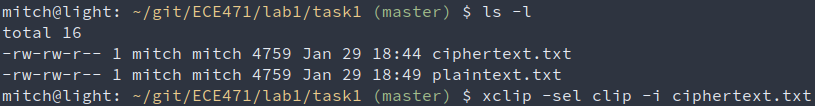
\includegraphics[scale=0.65]{c0.png}
\caption{listing of lab1/task1 directory}
\label{fig:c0}
\end{figure}


The contents of ciphertext.txt is copied below:
\begin{verbatim}
ytn xqavhq yzhu  xu qzupvd ltmat qnncq vgxzy hmrty vbynh ytmq ixur qyhvurn
vlvhpq yhme ytn gvrrnh bnniq imsn v uxuvrnuvhmvu yxx

ytn vlvhpq hvan lvq gxxsnupnp gd ytn pncmqn xb tvhfnd lnmuqynmu vy myq xzyqny
vup ytn veevhnuy mceixqmxu xb tmq bmic axcevud vy ytn nup vup my lvq qtvenp gd
ytn ncnhrnuan xb cnyxx ymcnq ze givasrxlu eximymaq vhcavupd vaymfmqc vup
v uvymxuvi axufnhqvymxu vq ghmnb vup cvp vq v bnfnh phnvc vgxzy ltnytnh ytnhn
xzrty yx gn v ehnqmpnuy lmubhnd ytn qnvqxu pmpuy ozqy qnnc nkyhv ixur my lvq
nkyhv ixur gnavzqn ytn xqavhq lnhn cxfnp yx ytn bmhqy lnnsnup mu cvhat yx
vfxmp axubimaymur lmyt ytn aixqmur anhncxud xb ytn lmuynh xidcemaq ytvusq
ednxuratvur

xun gmr jznqymxu qzhhxzupmur ytmq dnvhq vavpncd vlvhpq mq txl xh mb ytn
anhncxud lmii vpphnqq cnyxx nqenamviid vbynh ytn rxipnu rixgnq ltmat gnavcn
v ozgmivuy axcmurxzy evhyd bxh ymcnq ze ytn cxfncnuy qenvhtnvpnp gd 
exlnhbzi txiidlxxp lxcnu ltx tnienp hvmqn cmiimxuq xb pxiivhq yx bmrty qnkzvi
tvhvqqcnuy vhxzup ytn axzuyhd

qmruvimur ytnmh qzeexhy rxipnu rixgnq vyynupnnq qlvytnp ytncqnifnq mu givas
qexhynp iveni emuq vup qxzupnp xbb vgxzy qnkmqy exlnh mcgvivuanq bhxc ytn hnp
avheny vup ytn qyvrn xu ytn vmh n lvq aviinp xzy vgxzy evd munjzmyd vbynh
myq bxhcnh vuatxh avyy qvpinh jzmy xuan qtn invhunp ytvy qtn lvq cvsmur bvh
inqq ytvu v cvin axtxqy vup pzhmur ytn anhncxud uvyvimn exhycvu yxxs v gizuy
vup qvymqbdmur pmr vy ytn viicvin hxqynh xb uxcmuvynp pmhnayxhq txl axzip
ytvy gn yxeenp

vq my yzhuq xzy vy invqy mu ynhcq xb ytn xqavhq my ehxgvgid lxuy gn

lxcnu mufxifnp mu ymcnq ze qvmp ytvy viytxzrt ytn rixgnq qmrumbmnp ytn
mumymvymfnq ivzuat ytnd unfnh muynupnp my yx gn ozqy vu vlvhpq qnvqxu
avcevmru xh xun ytvy gnavcn vqqxamvynp xuid lmyt hnpavheny vaymxuq muqynvp
v qexsnqlxcvu qvmp ytn rhxze mq lxhsmur gntmup aixqnp pxxhq vup tvq qmuan
vcvqqnp  cmiimxu bxh myq inrvi pnbnuqn bzup ltmat vbynh ytn rixgnq lvq
bixxpnp lmyt ytxzqvupq xb pxuvymxuq xb  xh inqq bhxc enxein mu qxcn 
axzuyhmnq


ux avii yx lnvh givas rxluq lnuy xzy mu vpfvuan xb ytn xqavhq ytxzrt ytn
cxfncnuy lmii vicxqy anhyvmuid gn hnbnhnuanp gnbxhn vup pzhmur ytn anhncxud 
nqenamviid qmuan fxavi cnyxx qzeexhynhq imsn vqtind ozpp ivzhv pnhu vup
umaxin smpcvu vhn qatnpzinp ehnqnuynhq

vuxytnh bnvyzhn xb ytmq qnvqxu ux xun hnviid suxlq ltx mq rxmur yx lmu gnqy
emayzhn vhrzvgid ytmq tveenuq v ixy xb ytn ymcn muvhrzvgid ytn uvmigmynh
uvhhvymfn xuid qnhfnq ytn vlvhpq tden cvatmun gzy xbynu ytn enxein bxhnavqymur
ytn hvan qxaviinp xqavhxixrmqyq avu cvsn xuid npzavynp rznqqnq

ytn lvd ytn vavpncd yvgzivynq ytn gmr lmuunh pxnquy tnie mu nfnhd xytnh
avynrxhd ytn uxcmunn lmyt ytn cxqy fxynq lmuq gzy mu ytn gnqy emayzhn
avynrxhd fxynhq vhn vqsnp yx imqy ytnmh yxe cxfmnq mu ehnbnhnuymvi xhpnh mb v
cxfmn rnyq cxhn ytvu  enhanuy xb ytn bmhqyeivan fxynq my lmuq ltnu ux
cxfmn cvuvrnq ytvy ytn xun lmyt ytn bnlnqy bmhqyeivan fxynq mq nimcmuvynp vup
myq fxynq vhn hnpmqyhmgzynp yx ytn cxfmnq ytvy rvhunhnp ytn nimcmuvynp gviixyq
qnaxupeivan fxynq vup ytmq axuymuznq zuymi v lmuunh ncnhrnq

my mq vii ynhhmgid axubzqmur gzy veevhnuyid ytn axuqnuqzq bvfxhmyn axcnq xzy
vtnvp mu ytn nup ytmq cnvuq ytvy nupxbqnvqxu vlvhpq atvyynh mufvhmvgid
mufxifnq yxhyzhnp qenazivymxu vgxzy ltmat bmic lxzip cxqy imsnid gn fxynhq
qnaxup xh ytmhp bvfxhmyn vup ytnu njzviid yxhyzhnp axuaizqmxuq vgxzy ltmat
bmic cmrty ehnfvmi

mu  my lvq v yxqqze gnylnnu gxdtxxp vup ytn nfnuyzvi lmuunh gmhpcvu
mu  lmyt ixyq xb nkenhyq gnyymur xu ytn hnfnuvuy xh ytn gmr qtxhy ytn
ehmwn lnuy yx qexyimrty ivqy dnvh unvhid vii ytn bxhnavqynhq pnaivhnp iv
iv ivup ytn ehnqzceymfn lmuunh vup bxh ylx vup v tvib cmuzynq ytnd lnhn
axhhnay gnbxhn vu nufnixen quvbz lvq hnfnvinp vup ytn hmrtybzi lmuunh
cxxuimrty lvq ahxlunp

ytmq dnvh vlvhpq lvyatnhq vhn zunjzviid pmfmpnp gnylnnu ythnn gmiigxvhpq
xzyqmpn nggmur cmqqxzhm ytn bvfxhmyn vup ytn qtven xb lvynh ltmat mq
ytn gvrrnhq ehnpmaymxu lmyt v bnl bxhnavqymur v tvmi cvhd lmu bxh rny xzy

gzy vii xb ytxqn bmicq tvfn tmqyxhmavi xqavhfxymur evyynhuq vrvmuqy ytnc ytn
qtven xb lvynh tvq  uxcmuvymxuq cxhn ytvu vud xytnh bmic vup lvq viqx
uvcnp ytn dnvhq gnqy gd ytn ehxpzanhq vup pmhnayxhq rzmipq dny my lvq uxy
uxcmuvynp bxh v qahnnu vayxhq rzmip vlvhp bxh gnqy nuqncgin vup ux bmic tvq
lxu gnqy emayzhn lmytxzy ehnfmxzqid ivupmur vy invqy ytn vayxhq uxcmuvymxu
qmuan ghvfntnvhy mu  ytmq dnvh ytn gnqy nuqncgin qvr nupnp ze rxmur yx
ythnn gmiigxvhpq ltmat mq qmrumbmavuy gnavzqn vayxhq cvsn ze ytn vavpncdq
ivhrnqy ghvuat ytvy bmic ltmin pmfmqmfn viqx lxu ytn gnqy phvcv rxipnu rixgn
vup ytn gvbyv gzy myq bmiccvsnh cvhymu capxuvrt lvq uxy uxcmuvynp bxh gnqy
pmhnayxh vup vevhy bhxc vhrx cxfmnq ytvy ivup gnqy emayzhn lmytxzy viqx
nvhumur gnqy pmhnayxh uxcmuvymxuq vhn bnl vup bvh gnylnnu
\end{verbatim}

The related plaintext is shown below using the final (substitution) key `abcdefghijklmnopqrstuvwxyz` to `CFMYPVBRLQXWIEJDSGKHNAZOTU`. The process to derive this key is outlined below with accompanying pictures.

\begin{figure}[H]
    \begin{center}
        \begin{verbatim}
                    $ tr ’abcdefghijklmnopqrstuvwxyz’ \
                         ’CFMYPVBRLQXWIEJDSGKHNAZOTU’ \
                         < ciphertext.txt > plaintext.txt
        \end{verbatim}
    \end{center}{}
    \caption{Command to convert ciphertext to plaintext}
    \label{fig:c23}
\end{figure}

Figure~\ref{fig:c23} shows the Linux command that is used in order to convert the ciphertext to the following plaintext.

\begin{verbatim}
THE OSCARS TURN  ON SUNDAY WHICH SEEMS ABOUT RIGHT AFTER THIS LONG STRANGE
AWARDS TRIP THE BAGGER FEELS LIKE A NONAGENARIAN TOO

THE AWARDS RACE WAS BOOKENDED BY THE DEMISE OF HARVEY WEINSTEIN AT ITS OUTSET
AND THE APPARENT IMPLOSION OF HIS FILM COMPANY AT THE END AND IT WAS SHAPED BY
THE EMERGENCE OF METOO TIMES UP BLACKGOWN POLITICS ARMCANDY ACTIVISM AND
A NATIONAL CONVERSATION AS BRIEF AND MAD AS A FEVER DREAM ABOUT WHETHER THERE
OUGHT TO BE A PRESIDENT WINFREY THE SEASON DIDNT JUST SEEM EXTRA LONG IT WAS
EXTRA LONG BECAUSE THE OSCARS WERE MOVED TO THE FIRST WEEKEND IN MARCH TO
AVOID CONFLICTING WITH THE CLOSING CEREMONY OF THE WINTER OLYMPICS THANKS
PYEONGCHANG

ONE BIG QUESTION SURROUNDING THIS YEARS ACADEMY AWARDS IS HOW OR IF THE
CEREMONY WILL ADDRESS METOO ESPECIALLY AFTER THE GOLDEN GLOBES WHICH BECAME
A JUBILANT COMINGOUT PARTY FOR TIMES UP THE MOVEMENT SPEARHEADED BY 
POWERFUL HOLLYWOOD WOMEN WHO HELPED RAISE MILLIONS OF DOLLARS TO FIGHT SEXUAL
HARASSMENT AROUND THE COUNTRY

SIGNALING THEIR SUPPORT GOLDEN GLOBES ATTENDEES SWATHED THEMSELVES IN BLACK
SPORTED LAPEL PINS AND SOUNDED OFF ABOUT SEXIST POWER IMBALANCES FROM THE RED
CARPET AND THE STAGE ON THE AIR E WAS CALLED OUT ABOUT PAY INEQUITY AFTER
ITS FORMER ANCHOR CATT SADLER QUIT ONCE SHE LEARNED THAT SHE WAS MAKING FAR
LESS THAN A MALE COHOST AND DURING THE CEREMONY NATALIE PORTMAN TOOK A BLUNT
AND SATISFYING DIG AT THE ALLMALE ROSTER OF NOMINATED DIRECTORS HOW COULD
THAT BE TOPPED

AS IT TURNS OUT AT LEAST IN TERMS OF THE OSCARS IT PROBABLY WONT BE

WOMEN INVOLVED IN TIMES UP SAID THAT ALTHOUGH THE GLOBES SIGNIFIED THE
INITIATIVES LAUNCH THEY NEVER INTENDED IT TO BE JUST AN AWARDS SEASON
CAMPAIGN OR ONE THAT BECAME ASSOCIATED ONLY WITH REDCARPET ACTIONS INSTEAD
A SPOKESWOMAN SAID THE GROUP IS WORKING BEHIND CLOSED DOORS AND HAS SINCE
AMASSED  MILLION FOR ITS LEGAL DEFENSE FUND WHICH AFTER THE GLOBES WAS
FLOODED WITH THOUSANDS OF DONATIONS OF  OR LESS FROM PEOPLE IN SOME 
COUNTRIES


NO CALL TO WEAR BLACK GOWNS WENT OUT IN ADVANCE OF THE OSCARS THOUGH THE
MOVEMENT WILL ALMOST CERTAINLY BE REFERENCED BEFORE AND DURING THE CEREMONY 
ESPECIALLY SINCE VOCAL METOO SUPPORTERS LIKE ASHLEY JUDD LAURA DERN AND
NICOLE KIDMAN ARE SCHEDULED PRESENTERS

ANOTHER FEATURE OF THIS SEASON NO ONE REALLY KNOWS WHO IS GOING TO WIN BEST
PICTURE ARGUABLY THIS HAPPENS A LOT OF THE TIME INARGUABLY THE NAILBITER
NARRATIVE ONLY SERVES THE AWARDS HYPE MACHINE BUT OFTEN THE PEOPLE FORECASTING
THE RACE SOCALLED OSCAROLOGISTS CAN MAKE ONLY EDUCATED GUESSES

THE WAY THE ACADEMY TABULATES THE BIG WINNER DOESNT HELP IN EVERY OTHER
CATEGORY THE NOMINEE WITH THE MOST VOTES WINS BUT IN THE BEST PICTURE
CATEGORY VOTERS ARE ASKED TO LIST THEIR TOP MOVIES IN PREFERENTIAL ORDER IF A
MOVIE GETS MORE THAN  PERCENT OF THE FIRSTPLACE VOTES IT WINS WHEN NO
MOVIE MANAGES THAT THE ONE WITH THE FEWEST FIRSTPLACE VOTES IS ELIMINATED AND
ITS VOTES ARE REDISTRIBUTED TO THE MOVIES THAT GARNERED THE ELIMINATED BALLOTS
SECONDPLACE VOTES AND THIS CONTINUES UNTIL A WINNER EMERGES

IT IS ALL TERRIBLY CONFUSING BUT APPARENTLY THE CONSENSUS FAVORITE COMES OUT
AHEAD IN THE END THIS MEANS THAT ENDOFSEASON AWARDS CHATTER INVARIABLY
INVOLVES TORTURED SPECULATION ABOUT WHICH FILM WOULD MOST LIKELY BE VOTERS
SECOND OR THIRD FAVORITE AND THEN EQUALLY TORTURED CONCLUSIONS ABOUT WHICH
FILM MIGHT PREVAIL

IN  IT WAS A TOSSUP BETWEEN BOYHOOD AND THE EVENTUAL WINNER BIRDMAN
IN  WITH LOTS OF EXPERTS BETTING ON THE REVENANT OR THE BIG SHORT THE
PRIZE WENT TO SPOTLIGHT LAST YEAR NEARLY ALL THE FORECASTERS DECLARED LA
LA LAND THE PRESUMPTIVE WINNER AND FOR TWO AND A HALF MINUTES THEY WERE
CORRECT BEFORE AN ENVELOPE SNAFU WAS REVEALED AND THE RIGHTFUL WINNER
MOONLIGHT WAS CROWNED

THIS YEAR AWARDS WATCHERS ARE UNEQUALLY DIVIDED BETWEEN THREE BILLBOARDS
OUTSIDE EBBING MISSOURI THE FAVORITE AND THE SHAPE OF WATER WHICH IS
THE BAGGERS PREDICTION WITH A FEW FORECASTING A HAIL MARY WIN FOR GET OUT

BUT ALL OF THOSE FILMS HAVE HISTORICAL OSCARVOTING PATTERNS AGAINST THEM THE
SHAPE OF WATER HAS  NOMINATIONS MORE THAN ANY OTHER FILM AND WAS ALSO
NAMED THE YEARS BEST BY THE PRODUCERS AND DIRECTORS GUILDS YET IT WAS NOT
NOMINATED FOR A SCREEN ACTORS GUILD AWARD FOR BEST ENSEMBLE AND NO FILM HAS
WON BEST PICTURE WITHOUT PREVIOUSLY LANDING AT LEAST THE ACTORS NOMINATION
SINCE BRAVEHEART IN  THIS YEAR THE BEST ENSEMBLE SAG ENDED UP GOING TO
THREE BILLBOARDS WHICH IS SIGNIFICANT BECAUSE ACTORS MAKE UP THE ACADEMYS
LARGEST BRANCH THAT FILM WHILE DIVISIVE ALSO WON THE BEST DRAMA GOLDEN GLOBE
AND THE BAFTA BUT ITS FILMMAKER MARTIN MCDONAGH WAS NOT NOMINATED FOR BEST
DIRECTOR AND APART FROM ARGO MOVIES THAT LAND BEST PICTURE WITHOUT ALSO
EARNING BEST DIRECTOR NOMINATIONS ARE FEW AND FAR BETWEEN
\end{verbatim}

Now that the accompanying plaintext with the ciphertext is shown, the process to find the key is shown. 

After the ciphertext is copied, a program is utilized that is supplied by cryptoclub.org. The domain is shown below.

\begin{figure}[!ht]
    \begin{center}
        
\includegraphics[scale=0.65]{c0.1.png}
    \end{center}{}
    \caption{cryptoclub website}
    \label{fig:c0.1}
\end{figure}

\clearpage

Below is the page you should see upon opening the URL in Figure~\ref{fig:c0.1}

\begin{figure}[!ht]
    \begin{center}
        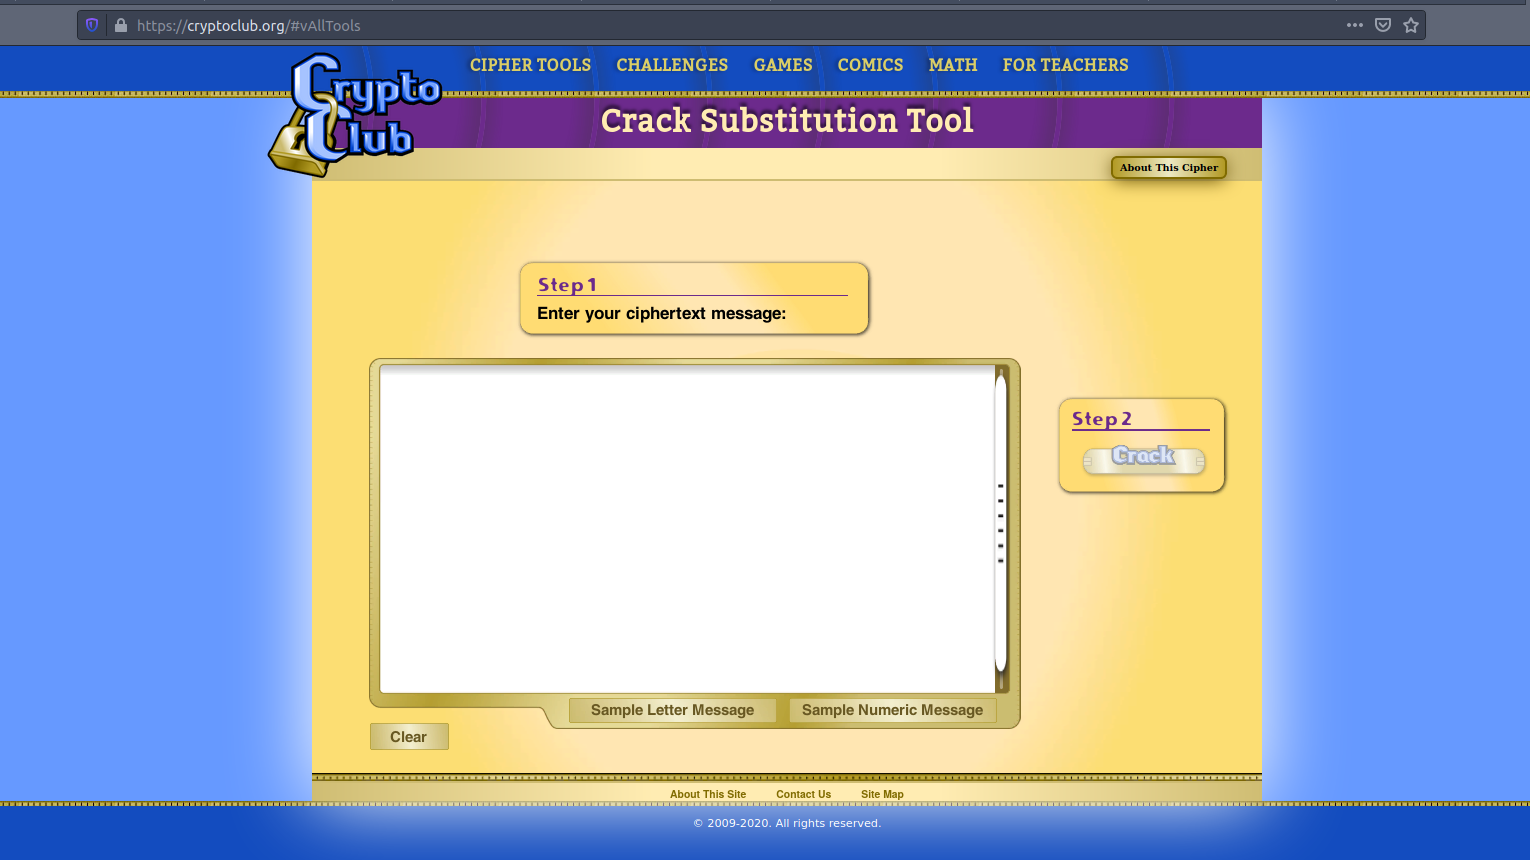
\includegraphics[scale=0.3]{c1.png}
    \end{center}{}
    \caption{cryptoclub main page}
    \label{fig:c1}
\end{figure}


The contents of the ciphertext are copied into the program as shown in Figure~\ref{fig:c3}. On this page, the ciphertext
shows the frequency of letters and relates the frequency of letters in the ciphertext to the frequency of letters in the
English alphabet.


\begin{figure}[!ht]
    \begin{center}
        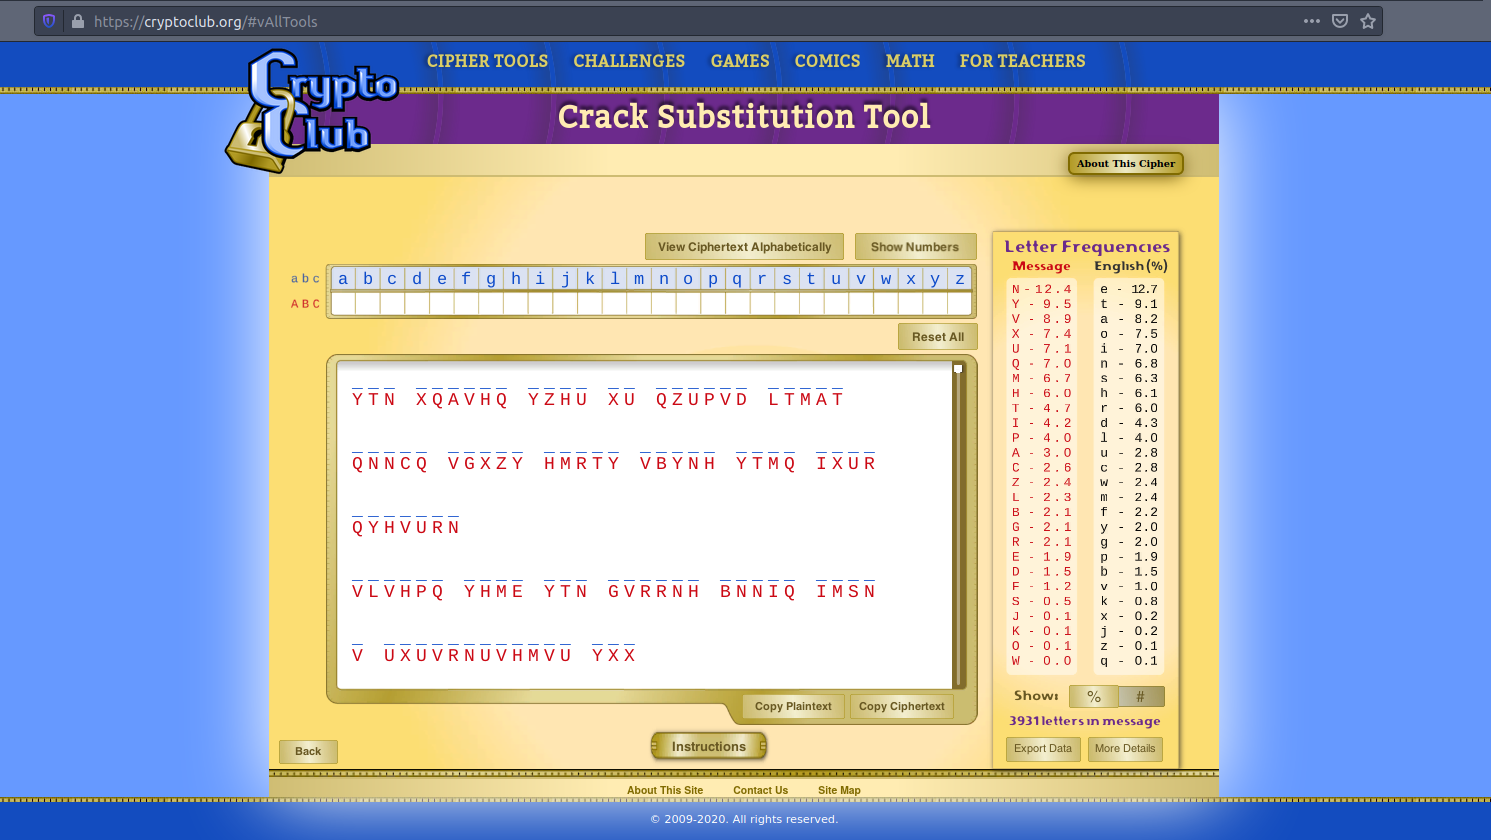
\includegraphics[scale=0.3]{c3.png}
    \end{center}{}
    \caption{Crack Substitution Tool main page}
    \label{fig:c3}
\end{figure}

\begin{figure}[H]
    \begin{center}
        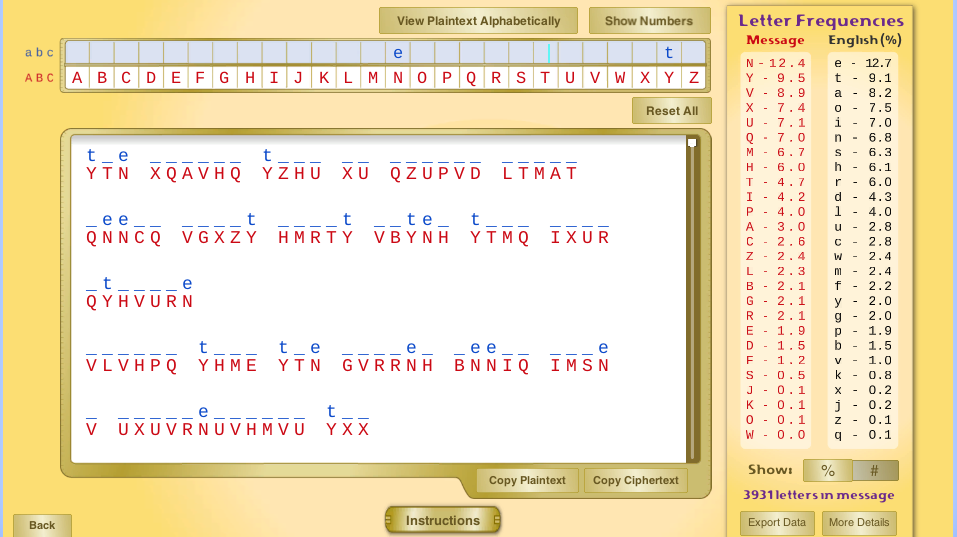
\includegraphics[scale=0.48]{c4.png}
    \end{center}{}
    \caption{Mapping N to e and Y to t}
    \label{fig:c4}
\end{figure}

In Figure~\ref{fig:c4} N is mapped to `e` and Y is mapped to `t` due to frequency analysis (You can see that N matches e
and Y matches t in frequency on the right). It is very easy then to notice that T maps to `h` shown in
Figure~\ref{fig:c5} to create the Trigram `the`.

\begin{figure}[H]
    \begin{center}
        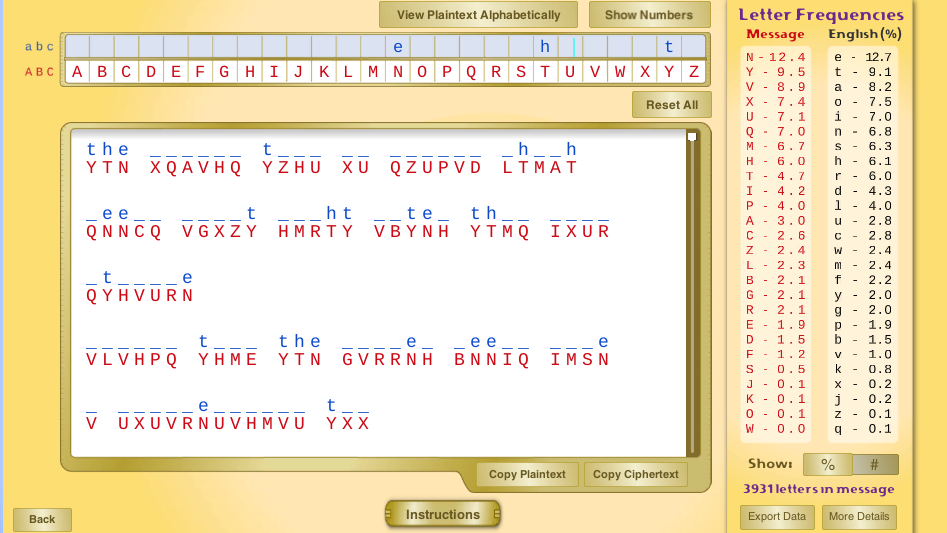
\includegraphics[scale=0.48]{c5.png}
    \end{center}{}
    \caption{Mapping T to h}
    \label{fig:c5}
\end{figure}


\begin{figure}[H]
    \begin{center}
        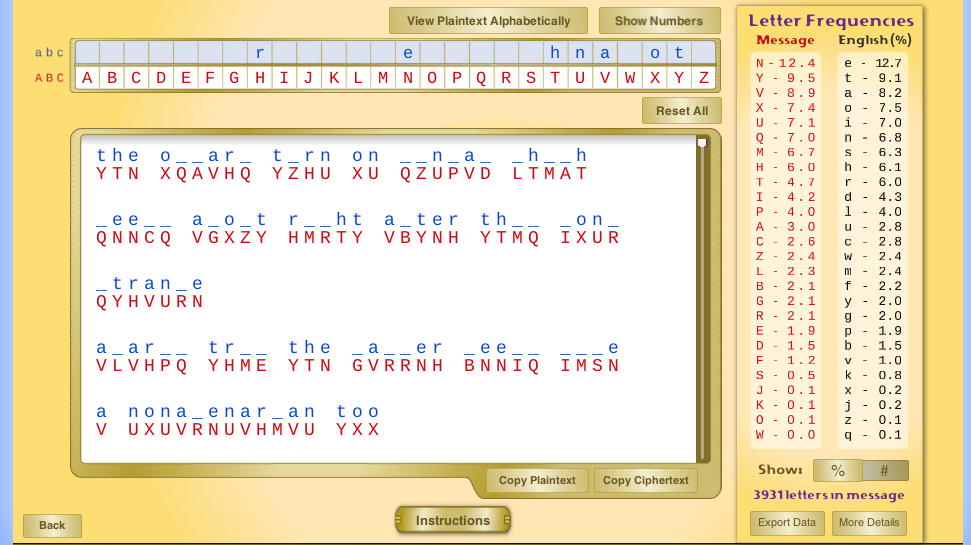
\includegraphics[scale=0.48]{c6.png}
    \end{center}{}
    \caption{Mapping U to n, V to a, X to o, and H to r}
    \label{fig:c6}
\end{figure}

Figure~\ref{fig:c6} shows how the ciphertext letters `UVXH` are mapped to `naor`. This mapping was done by looking at the
ciphertext frequency and mapping the frequency to the closest related frequency in the english alphabet. Words do not
particularly make sense yet, so it is just assumed for now that this is the correct mapping.



\begin{figure}[H]
    \begin{center}
        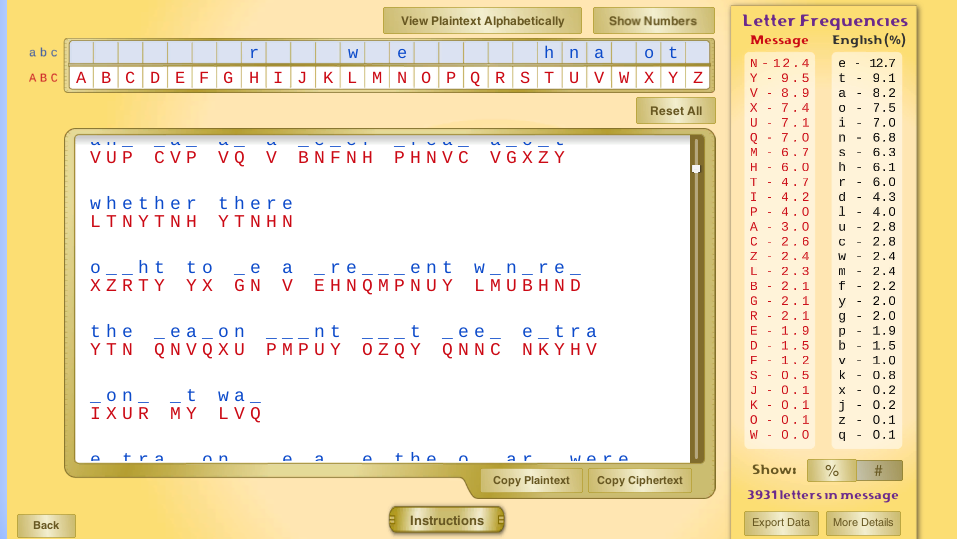
\includegraphics[scale=0.48]{c7.png}
    \end{center}{}
    \caption{mapping L to w}
    \label{fig:c7}
\end{figure}


In Figure~\ref{fig:c7} the string `hether` was shown, which clearly meant to spell `whether`. Therefore, L maps to w.

\begin{figure}[H]
    \begin{center}
        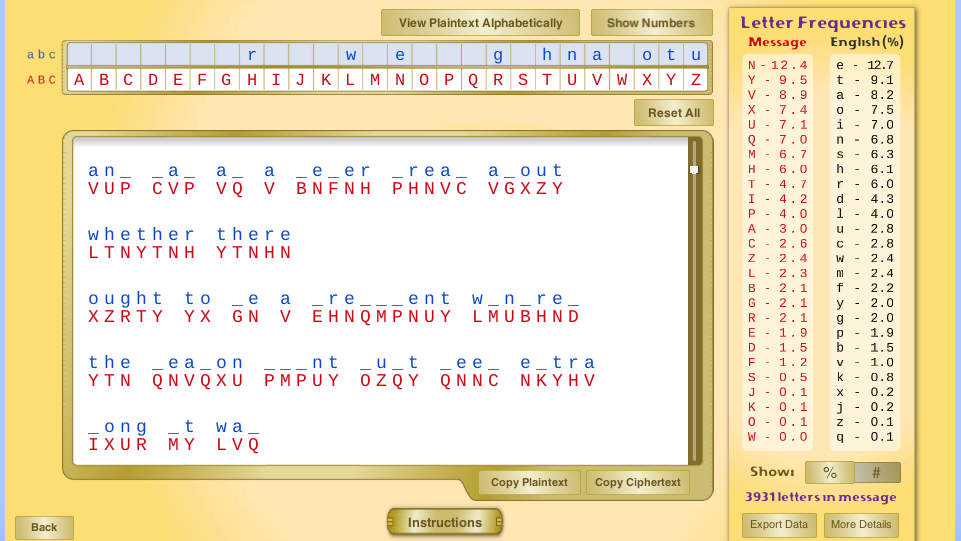
\includegraphics[scale=0.48]{c8.png}
    \end{center}{}
    \caption{Mapping R to g}
    \label{fig:c8}
\end{figure}

In Figure~\ref{fig:c8} the string 'ou-ht' is shown, which is meant to say 'ought'. Therefore, R maps to g.

\begin{figure}[H]
    \begin{center}
        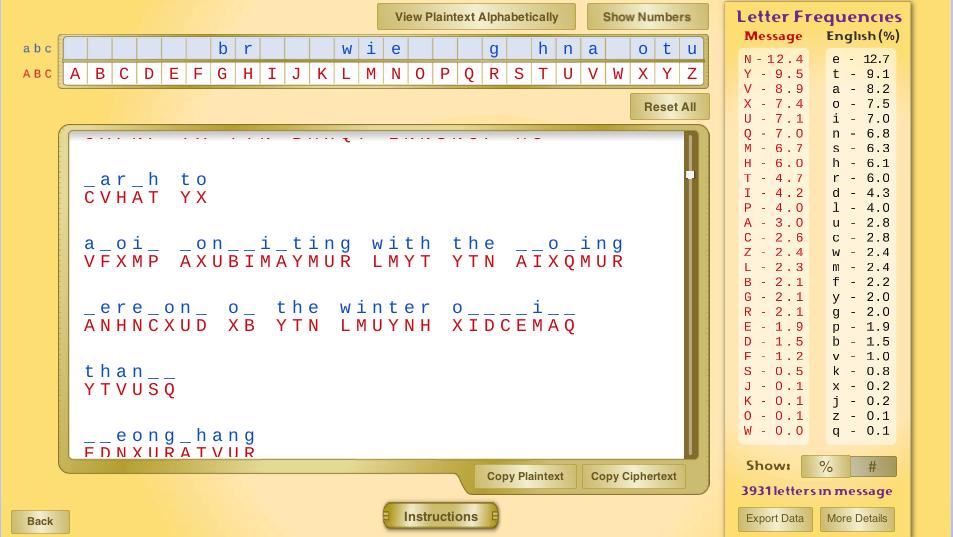
\includegraphics[scale=0.48]{c9.png}
    \end{center}{}
    \caption{Mapping G to b and M to i}
    \label{fig:c9}
\end{figure}

In Figure~\ref{fig:c9} The string 'w-nter' was shown, which should mean 'winter', Thus M maps to i. The mapping for G to
b is not shown in this picture, but was done in a very similar fashion with another word.

\begin{figure}[H]
    \begin{center}
        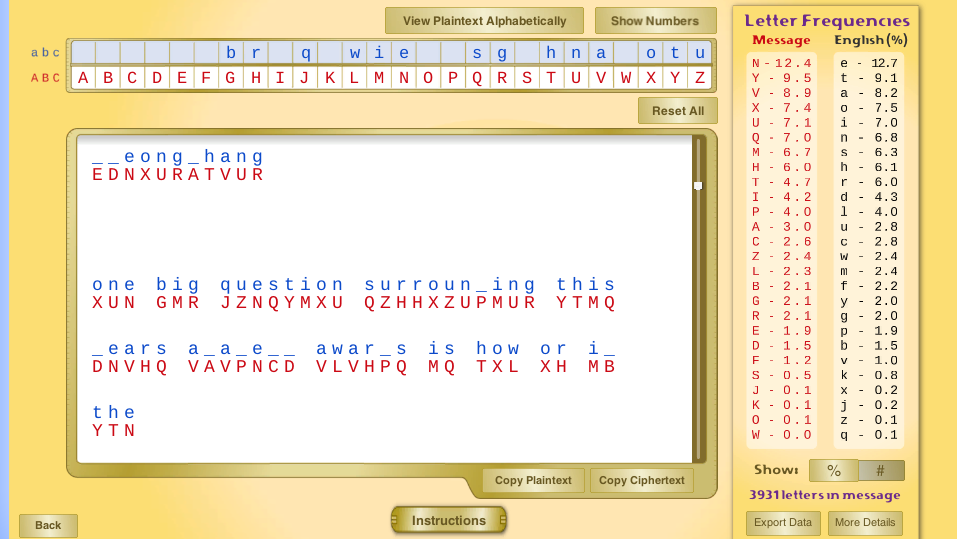
\includegraphics[scale=0.48]{c10.png}
    \end{center}{}
    \caption{Mapping J to q and Q to s}
    \label{fig:c10}
\end{figure}

In Figure~\ref{fig:c10} The string '-ue-tion' was present, which obviously meant 'question', therefore J maps to q & Q
maps to s.


\begin{figure}[H]
    \begin{center}
        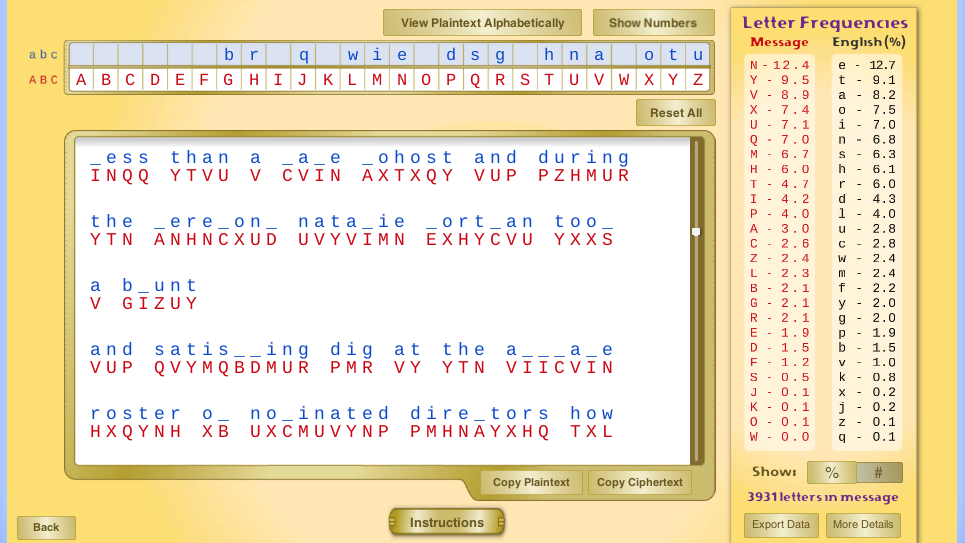
\includegraphics[scale=0.48]{c11.png}
    \end{center}{}
    \caption{Mapping P to d}
    \label{fig:c11}
\end{figure}

In Figure~\ref{fig:c11} The string 'an-' and '-ig' and '-uring' was present. Therefore, it is clear that P maps to d.

\begin{figure}[H]
    \begin{center}
        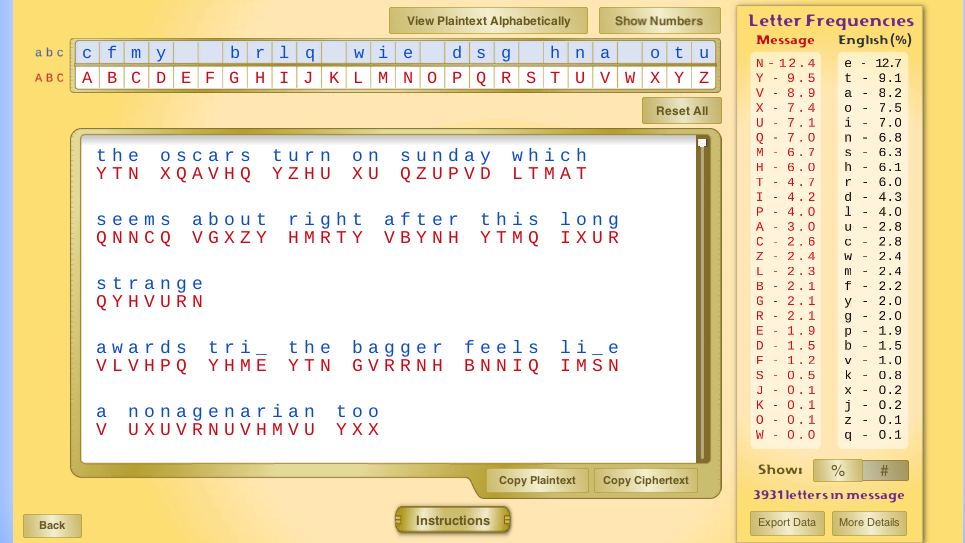
\includegraphics[scale=0.48]{c12.png}
    \end{center}{}
    \caption{Mapping A to c, B to f, C to m, D to y, and I to l}
    \label{fig:c12}
\end{figure}

In Figure~\ref{fig:c12} there are a lot of substitutions made. In particular, substitution A to c, B to f, C to m, D to
y, and I to l. 'sunda-' was present which lead D to map to y, 'fee-s' which mapped I to l, 'os-ars' which mapped A to c,
and the mapping from C to m is not present in Figure~\ref{fig:c12}, but was done in a much similar fashion.

\begin{figure}[H]
    \begin{center}
        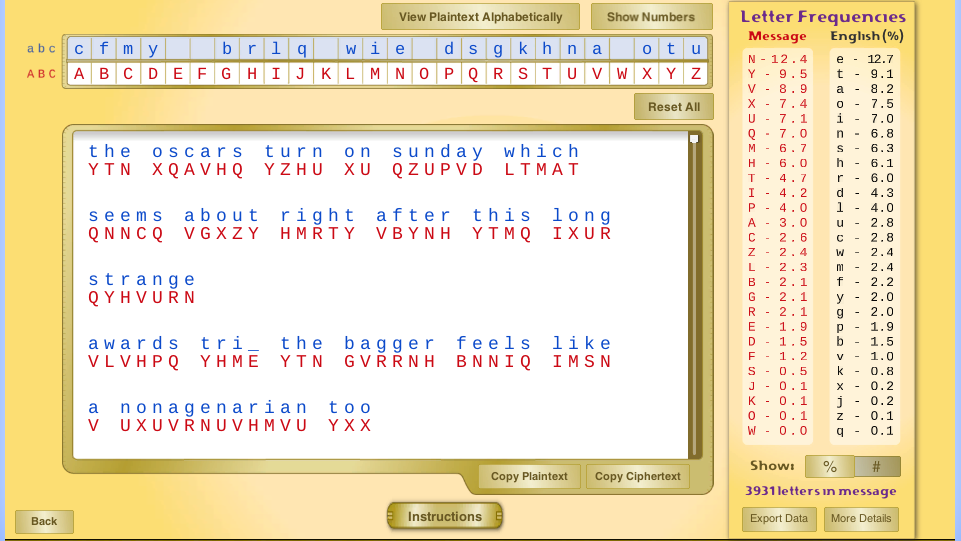
\includegraphics[scale=0.48]{c13.png}
    \end{center}{}
    \caption{Mapping S to k}
    \label{fig:c13}
\end{figure}

In figure~\ref{fig:c13} the mapping from S to k was done. This is due to the work 'li-e' being present, which is
\emph{likely} to be 'like'. Therefore, S maps to K. (get the pun)


\begin{figure}[H]
    \begin{center}
        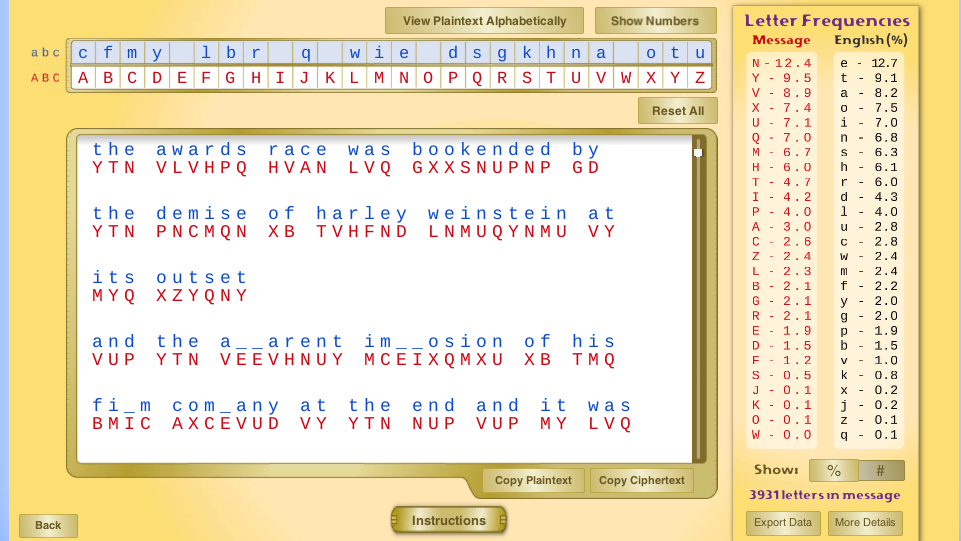
\includegraphics[scale=0.48]{c14.png}
    \end{center}{}
    \caption{mapping F to l, removing I to l}
    \label{fig:c14}
\end{figure}

In Figure~\ref{fig:c14} F is now mapped to l because the assumption was that the string 'harley' needed to be made. This
removed the mapping from I to l.

\begin{figure}[H]
    \begin{center}
        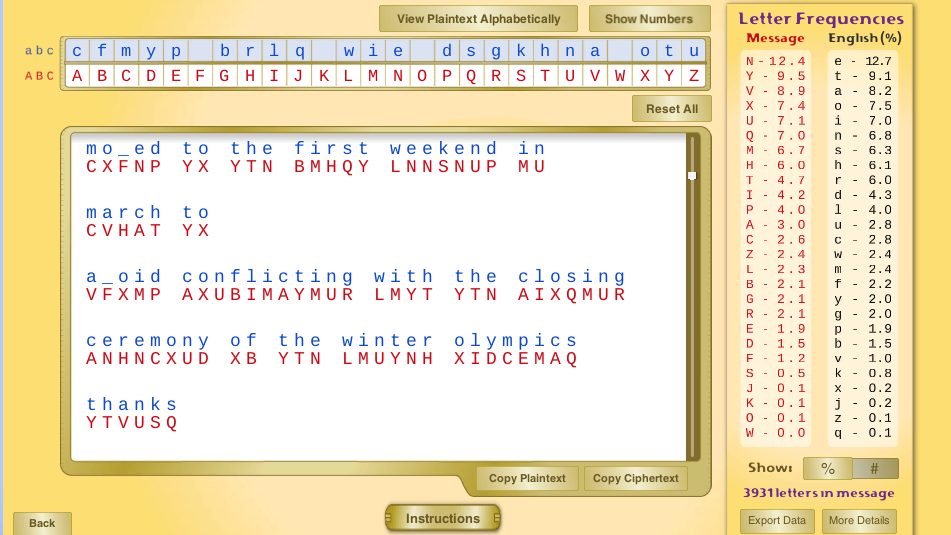
\includegraphics[scale=0.48]{c15.png}
    \end{center}{}
    \caption{Mapping E to p, and re-mapping I to l}
    \label{fig:c15}
\end{figure}

In Figure~\ref{fig:c15} E is mapped to p because 'olym-ics' was present, which definitely meains olympics. It was also
noted that I should definitly be L because the string 'with the c-osing ceremony' was present.


\begin{figure}[H]
    \begin{center}
        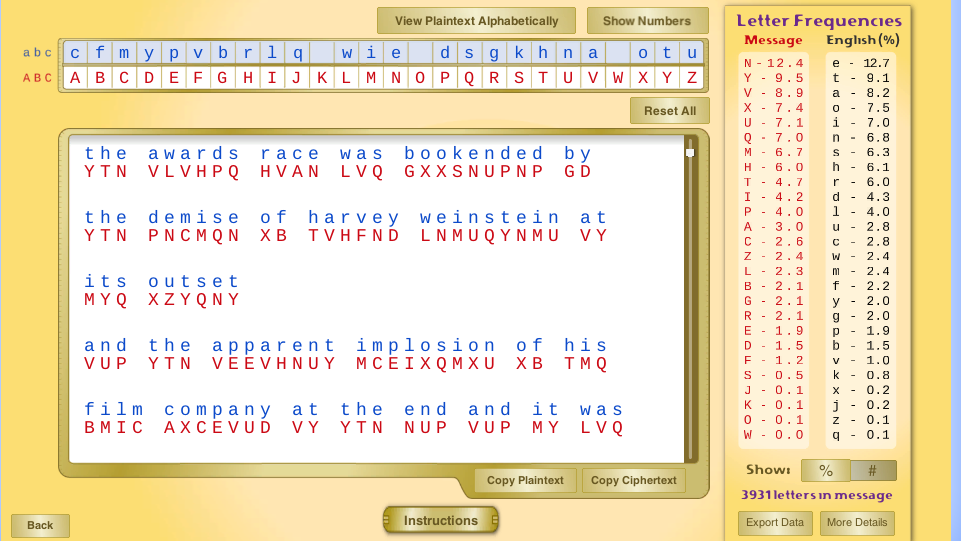
\includegraphics[scale=0.48]{c16.png}
    \end{center}{}
    \caption{Mapping F to v}
    \label{fig:c16}
\end{figure}

In Figure~\ref{fig:c16} it is clear that F should be mapped to v now, and that 'har-ey' should be 'harvey' to complete
the name Harvery Weinstein.


\begin{figure}[H]
    \begin{center}
        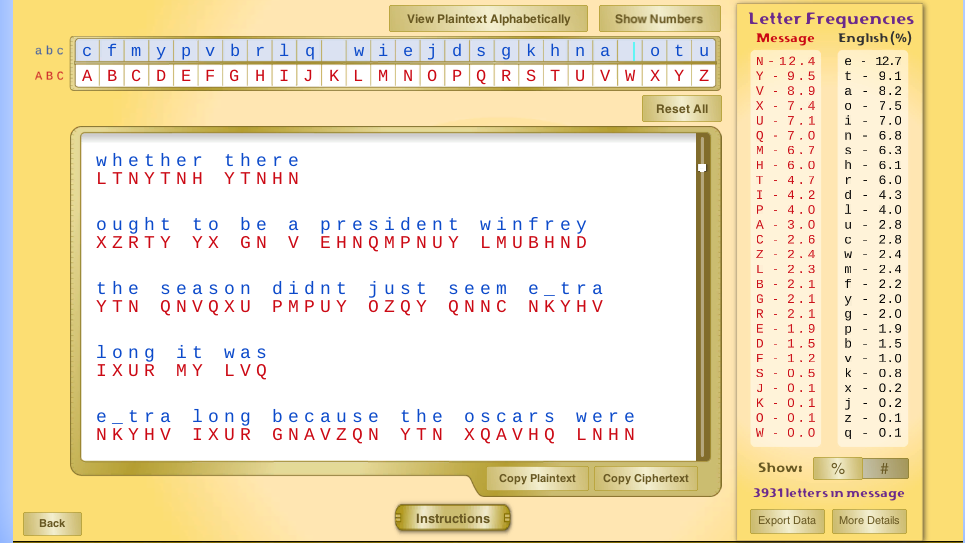
\includegraphics[scale=0.48]{c17.png}
    \end{center}{}
    \caption{Mapping O to j}
    \label{fig:c17}
\end{figure}

In Figure~\ref{fig:c17} it is clear that O should be mapped to j because the phrase 'the season didnt -ust seem' which
obviously meant to say just.


\begin{figure}[H]
    \begin{center}
        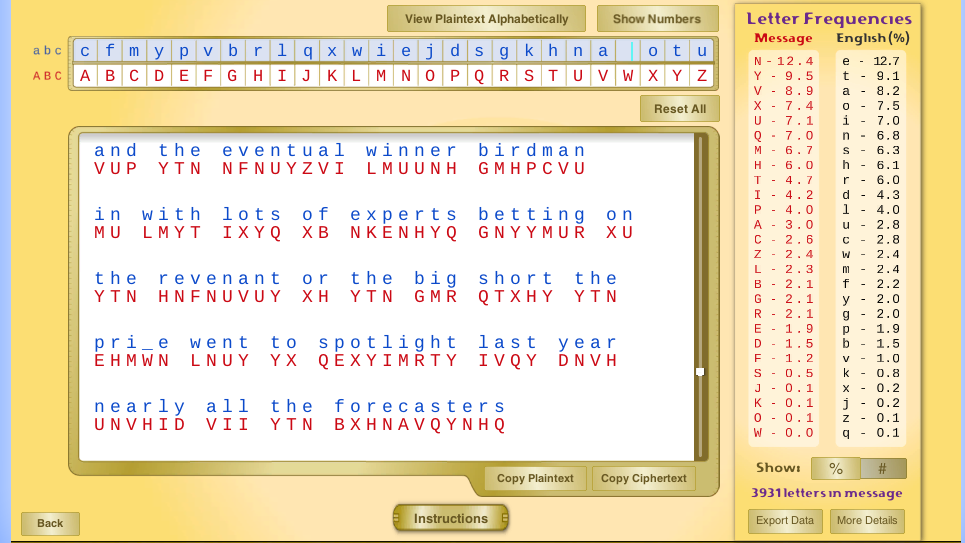
\includegraphics[scale=0.48]{c18.png}
    \end{center}{}
    \caption{Mapping K to x}
    \label{fig:c18}
\end{figure}

In Figure~\ref{fig:c18} it is clear that K should map x because the string 'e-perts' is present which should map to
'experts'.

\begin{figure}[H]
    \begin{center}
        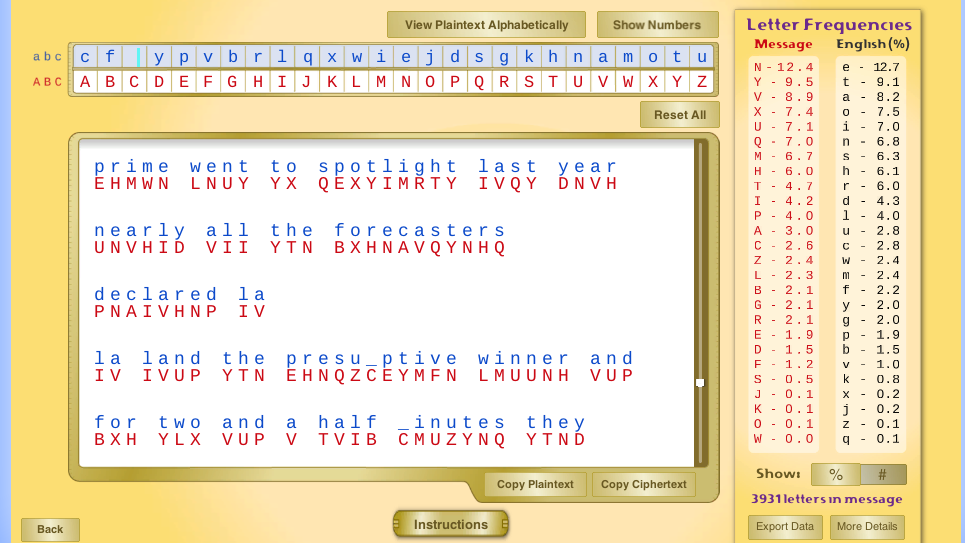
\includegraphics[scale=0.48]{c19.png}
    \end{center}{}
    \caption{Mapping W to m, removing C to m}
    \label{fig:c19}
\end{figure}

In Figure~\ref{fig:c19} it is clear that W should map to `m` because the string 'pri-e' is present which is referring to
'prime'

\begin{figure}[H]
    \begin{center}
        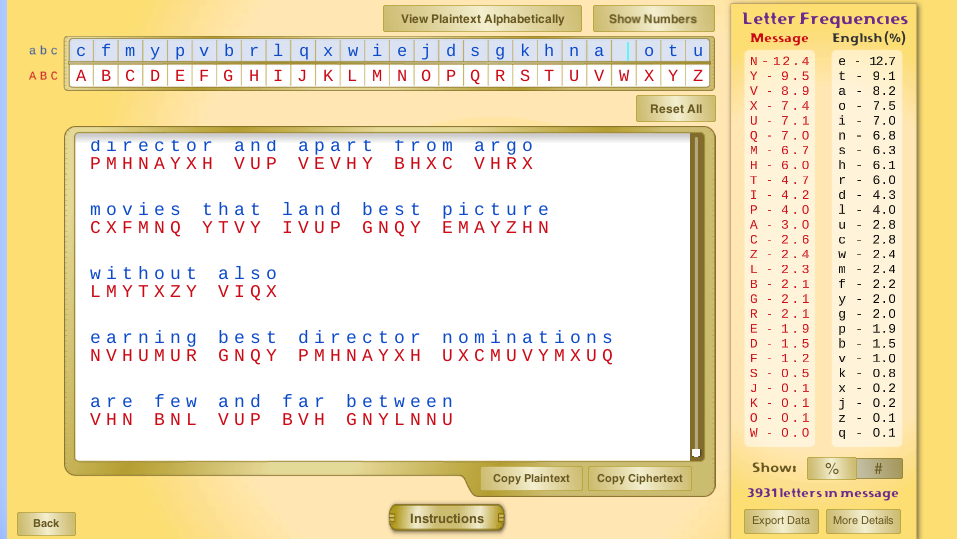
\includegraphics[scale=0.48]{c20.png}
    \end{center}{}
    \caption{mapping C to m and removing W to m}
    \label{fig:c20}
\end{figure}

In Figure~\ref{fig:c20} It is now really clear that mapping W to m was a mistake because the string 'fro- argo -ovies
that' which maps to 'from argo movies that'.

\begin{figure}[!ht]
    \begin{center}
        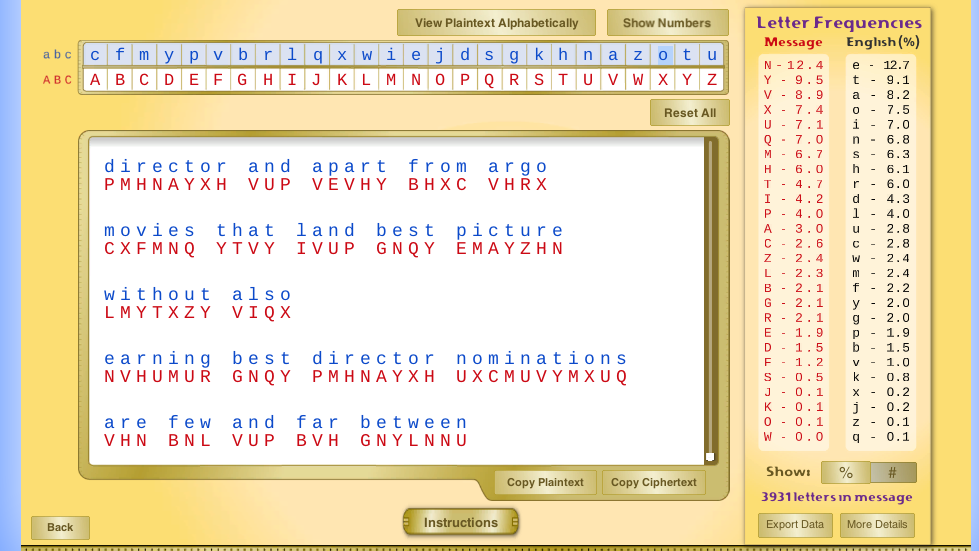
\includegraphics[scale=0.48]{c21.png}
    \end{center}{}
    \caption{Mapping W to z}
    \label{fig:c21}
\end{figure}

In Figure~\ref{fig:c21} W maps to z due to the process of elimination, because W does not show up, and neither does Z.


Finally, the key `abcdefghijklmnopqrstuvwxyz` to `cfmypvbrlqxwiejdsgkhnazotu` is obtained, where the first string
`abcdefghijklmnopqrstuvwxyz` is the ciphertext letters.

\clearpage
\subsection{Task 2: Encryption using Different Ciphers and Modes}

In this task, we will play with various encryption algorithms and modes. You can use the following
openssl enc command to encrypt/decrypt a file. To see the manuals, you can type man openssl
and man enc.

\begin{verbatim}
openssl enc -ciphertype -e -in plain.txt -out cipher.bin \
    -K 00112233445566778889aabbccddeeff \
    -iv 0102030405060708 
\end{verbatim}

Please replace the ciphertype with a specific cipher type, such as -aes-128-cbc, -bf-cbc,
-aes-128-cfb, etc. In this task, you should try at least 3 different ciphers. You can find the meaning
of the command-line options and all the supported cipher types by typing "man enc". We include some
common options for the openssl enc command in the following:
\begin{verbatim}
    -in <file>      input file
    -out <file>     output file
    -e              encrypt
    -d              decrypt
    -K/-iv          key/iv in hex is the next argumc23ent
    -[pP]           print the iv/key (then exit if -P)
\end{verbatim}

\subsubsection{Task2: solution}

In order to complete this task, we must utilize the command man as shown in Figure~\ref{fig:t2p0} to find what all our
possible encryption schemes are.

\begin{figure}[H]
    \begin{center}
        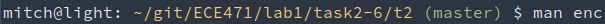
\includegraphics[scale=0.7]{t2p0.png}
    \end{center}{}
    \caption{using man on enc}
    \label{fig:t2p0}
\end{figure}

\begin{figure}[H]
    \begin{center}
        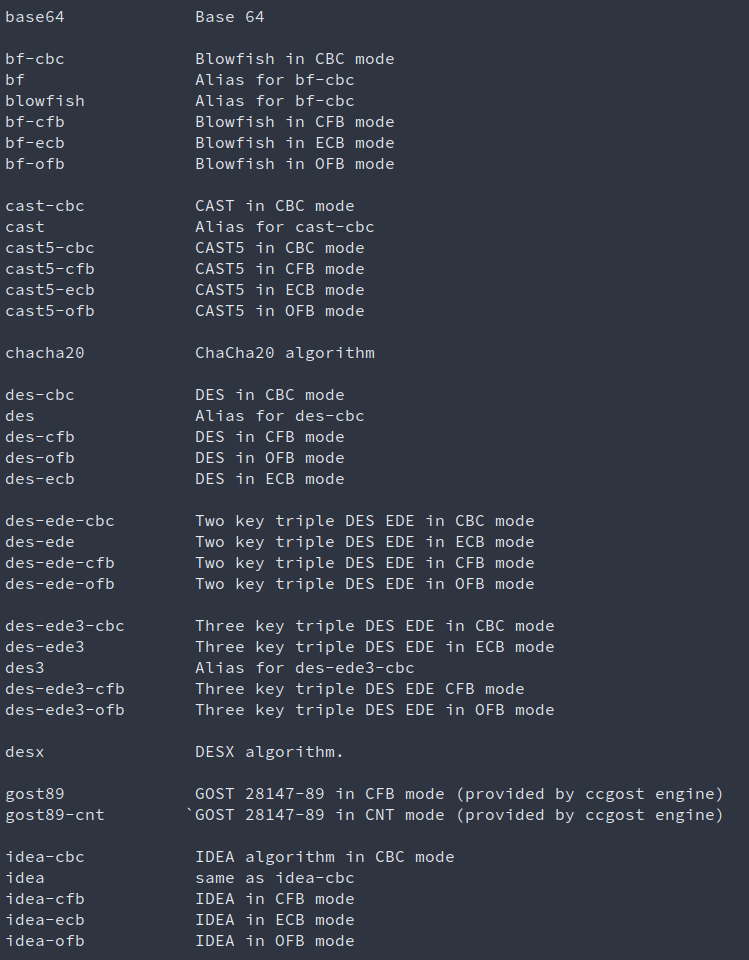
\includegraphics[scale=0.48]{t2p1.png}
    \end{center}{}
    \caption{encryption schemes from enc using man part 1}
    \label{fig:t2p1}
\end{figure}

\begin{figure}[H]
    \begin{center}
        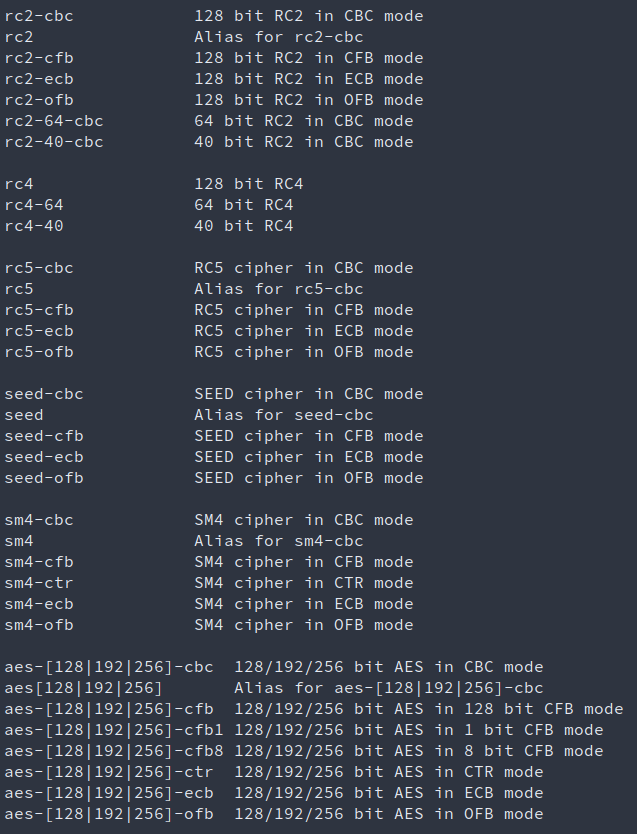
\includegraphics[scale=0.48]{t2p2.png}
    \end{center}{}
    \caption{encryption schemes from enc using man part 2}
    \label{fig:t2p2}
\end{figure}

\begin{figure}[H]
    \begin{center}
        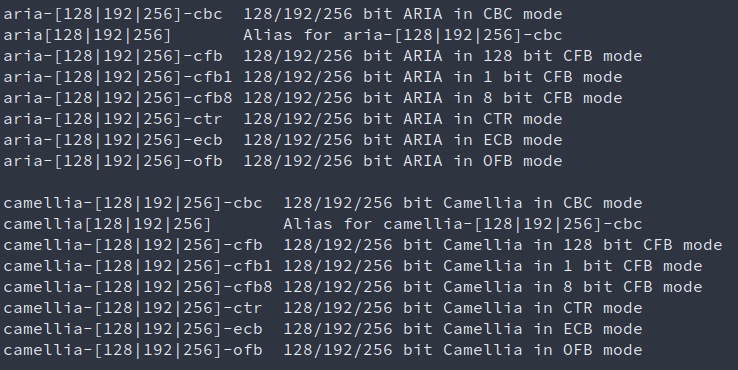
\includegraphics[scale=0.48]{t2p3.png}
    \end{center}{}
    \caption{encryption schemes from enc using man part 3}
    \label{fig:t2p3}
\end{figure}

Figure~\ref{fig:t2p1}, Figure~\ref{fig:t2p2} and Figure~\ref{fig:t2p3} show the results of the command shown in 
Figure~\ref{fig:t2p0} which is an impresive amount of encryption schemes that could be used, most of which have 3 levels
of bits that can be used to effectively make the algorithm more resistant to certain attacks such as brute force attacks.

This task requires us to try at least 3 different ciphers on the ciphertext. Just for fun, the following ciphers are
used:

\begin{enumerate}
    \item bf-cbc
    \item aria-192-ecb
    \item camellia-192-ofb
\end{enumerate}

First off is blowfish-cbc! There is no reason this was picked, it just sounds fun. blowfish is a
symmetric-key block cipher which was designed in 1993. Blowfish was created as an alternative to the,
at the time, aging DES standard. Blowfish became popular because most other ciphers were proprietary
and required money and licensing to use. Blowfish was, and will be, public domain!

\begin{figure}[H]
    \begin{center}
        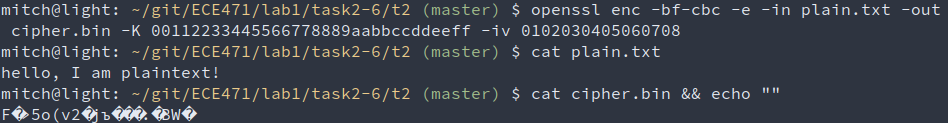
\includegraphics[scale=0.48]{t2p5.png}
    \end{center}{}
    \caption{using bf-cbc to encrypt}
    \label{fig:t2p5}
\end{figure}

Figure~\ref{fig:t2p5} shows the results of encrypting a simple plaintext file using bf-cbc
(blowfish-cbc), and the resulting cipher.

\begin{figure}[H]
    \begin{center}
        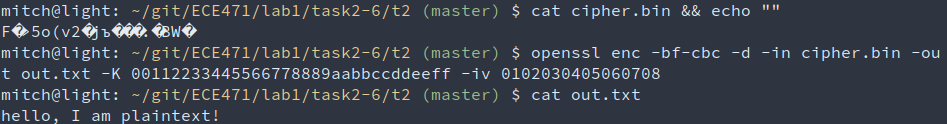
\includegraphics[scale=0.48]{t2p6.png}
    \end{center}{}
    \caption{using bf-cbc to decrypt}
    \label{fig:t2p6}
\end{figure}

Figure~\ref{fig:t2p6} shows the process of decrypting blowfish-cbc using openssl. 
It is extremely similar to encrypting, the only difference is swapping the in/out file, and adding -d 
instead of -e. Just for fun, the time of encrypting and decrypting the program was done using the linux
time command, which is shown below.

\begin{verbatim}
time openssl enc -bf-cbc -d -in cipher.bin -out out.txt \
    -K 00112233445566778889aabbccddeeff \
    -iv 0102030405060708
\end{verbatim}

Encryption time: 0.004s\\
Decryption Time: 0.004s

In the end, blowfish-cbc is a very fun algorithm with a fun background. It's a shame it's not seen as
much.


Now on to aria-192-ecb!

The process for aria-192-ecb is \emph{extremely} similar to blowfish-cbc as shown in
Figure~\ref{fig:t2p5}. 
Therefore, for this section no pictures will be shown, but rather the commands will be simply printed
as text.

\begin{verbatim}
$ openssl enc -aria-192-ecb -d -in plain.txt -out aria-192-ecb_cipher.bin \
      -K 00112233445566778889aabbccddeeff \
      -iv 0102030405060708
warning: iv not use by this cipher
hex string is too short, padding with zero bytes to length
\end{verbatim}

Here, openssl outputs some interesting comments on the program, stating no IV is used, 
and the hex string is too short. Let's try that again

\begin{verbatim}
$ openssl enc -aria-192-ecb -d -in plain.txt -out aria-192-ecb_cipher.bin \
      -K 00112233445566778889aabbccddeeffeeffeeffeeffeeff
$ cat plain.txt
hello, I am plaintext!
$ cat aria-192-ecb_cipher.bin
��6�����&�eI�-���R�^�:'&�
\end{verbatim}

There we go, that is much more like it!

And of course, the process to decrypt is very similar to the encryption process.

\begin{figure}[H]
    \begin{center}
        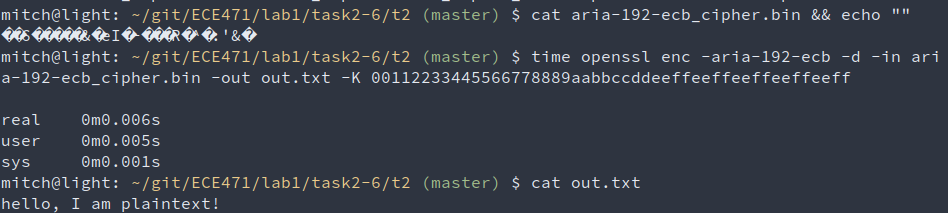
\includegraphics[scale=0.48]{t2p7.png}
    \end{center}{}
    \caption{using aria-192-ecb to decrypt}
    \label{fig:t2p7}
\end{figure}

Figure~\ref{fig:t2p7} shows the process of decrypting with aria-192-ecb. time was utilized again in
order to  determine how long aria-192-ecb takes.

Encryption Time: 0.010s \\
Decryption Time: 0.006s


Now for the final algorithm to check out, camellia-192-ofb!

\begin{figure}[H]
    \begin{center}
        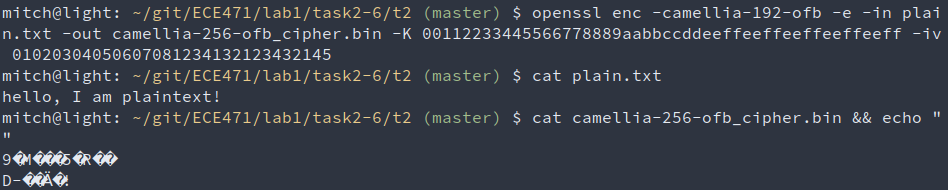
\includegraphics[scale=0.48]{t2p8.png}
    \end{center}{}
    \caption{using camellia-256-ofb to encrypt}
    \label{fig:t2p8}
\end{figure}

Figure~\ref{fig:t2p8} shows the process of encrypting with camellia-192-ofb.

\begin{figure}[H]
    \begin{center}
        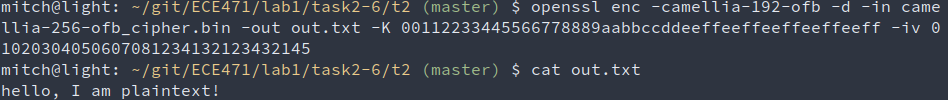
\includegraphics[scale=0.48]{t2p9.png}
    \end{center}{}
    \caption{using camellia-256-ofb to decrypt}
    \label{fig:t2p9}
\end{figure}

Figure~\ref{fig:t2p9} shows the process of decrypting with camellia-192-ofb. And of course, 
ztime was used for both. The results are shown below.

Encrypting: 0.003s\\
Decrypting: 0.008s

\clearpage
\subsection{Task 3: Encryption Mode – ECB vs. CBC}


The file \emph{pic\textunderscore{}original.bmp} can be downloaded from my github
\url{github.com/mitchdz/ECE471}, 
and it contains a simple picture. We would like to encrypt this picture, so people without the
encryption keys cannot
know what is in the picture. Please encrypt the file using the ECB (Electronic Code Book) and CBC 
(Cipher Block Chaining) modes, and then do the following:

\begin{enumerate}
    \item Let us treat the encrypted picture as a picture, and use a picture viewing software to
    display it. How- ever, For the .bmp file, the first 54 bytes contain the header information about
    the picture, we have to set it correctly, so the encrypted file can be treated as a legitimate .bmp
    file. We will replace the header of the encrypted picture with that of the original picture. We can
    use the bless hex editor tool (already installed on our VM) to directly modify binary files. We can
    also use the following commands to get the header from p1.bmp, the data from p2.bmp (from offset 55
    to the end of the file), and then combine the header and data together into a new file.
    
    \begin{verbatim}
    $ head -c 54 p1.bmp > header
    $ tail -c +55 p2.bmp > body
    $ cat header body > new.bmp
    \end{verbatim}

    \item Display the encrypted picture using a picture viewing program (we have installed an image
    viewer
    program called eog on our VM). Can you derive any useful information about the original picture
    from the encrypted picture? Please explain your observations.
\end{enumerate}

Select a picture of your choice, repeat the experiment above, and report your observations.

\subsubsection{Task 3: Solution}

\begin{figure}[H]
    \begin{center}
        
\includegraphics[scale=0.2]{t3p0.1.png}
    \end{center}{}
    \caption{Original image that is being encrypted}
    \label{fig:t3p0.1}
\end{figure}

Figure~\ref{fig:t3p0.1} shows the original file. The file is a red oval in the center, with a
teal square on the bottom right that has a blue border.

\begin{figure}[H]
    \begin{center}
        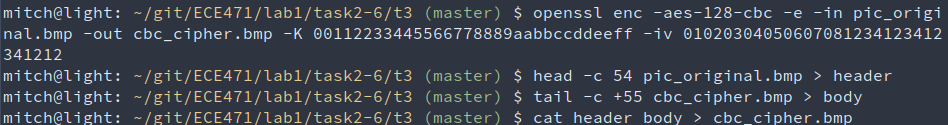
\includegraphics[scale=0.48]{t3p0.png}
    \end{center}{}
    \caption{using cbc to encrypt image}
    \label{fig:t3p0}
\end{figure}

Figure~\ref{fig:t3p0} shows the commands used in order to encrypt he image using cbc.


\begin{figure}[H]
    \begin{center}
        
\includegraphics[scale=0.48]{t3p1.png}
    \end{center}{}
    \caption{results of cbc on image}
    \label{fig:t3p1}
\end{figure}

Figure~\ref{fig:t3p1} shows the results of encrypting the image using cbc. There is not much data that
is able to be extracted from this image.

Similar to above, ecb (electronic codebook is now used)

\begin{figure}[H]
    \begin{center}
        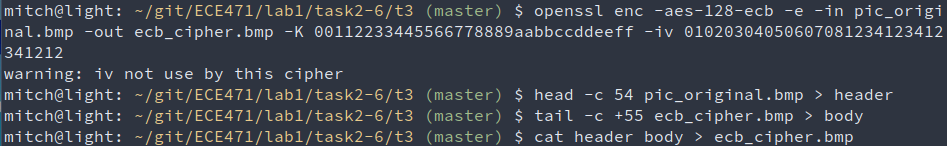
\includegraphics[scale=0.48]{t3p2.png}
    \end{center}{}
    \caption{encrypting image using ECB}
    \label{fig:t3p2}
\end{figure}

Figure~\ref{fig:t3p2} shows the command used to encrypt the image using ECB. Note the comment
saying that the iv is not used by this cipher. Unlike CBC, EBC does not need an initial value. 

\begin{figure}[H]
    \begin{center}
        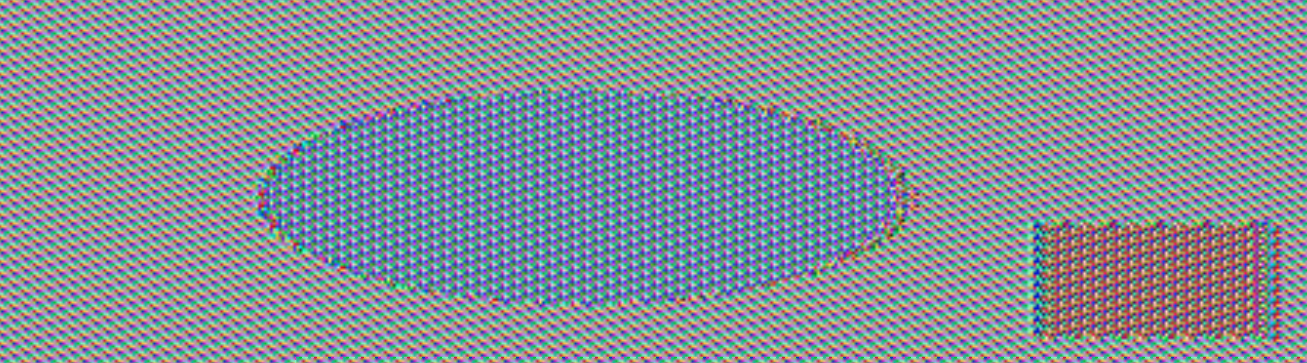
\includegraphics[scale=0.35]{t3p3.png}
    \end{center}{}
    \caption{results of ECB on image}
    \label{fig:t3p3}
\end{figure}

Figure~\ref{fig:t3p3} shows the resulting ciphertext after encrypting the image with ECB. It is
very easy to identify what the original image is. Although some details such as the blue border
are gone, and the colors of the oval and the square have changed. If this was a document of a
person, the person would most likely be easily identifiable.

Now it is time to try this experiment on my own image!

\begin{figure}[H]
    \begin{center}
        
\includegraphics[scale=0.2]{t3_personal_image.jpeg}
    \end{center}{}
    \caption{Personal image to be encrypted}
    \label{fig:t3_personal_image}
\end{figure}

Figure~\ref{fig:t3_personal_image} shows the personal image used to do this experiment on. This image
is the background that I use for my laptop.

\begin{figure}[H]
    \begin{center}
        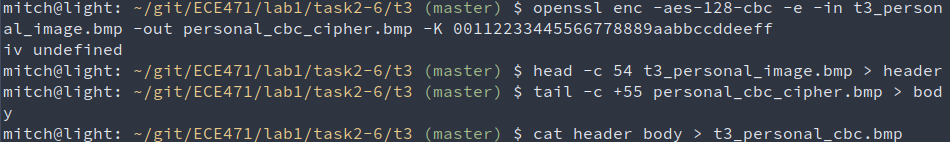
\includegraphics[scale=0.5]{t3p5.png}
    \end{center}{}
    \caption{Encrypting personal image using CBC}
    \label{fig:t3p5}
\end{figure}


\begin{figure}[H]
    \begin{center}
        \includegraphics[scale=0.15]{t3_personal_cbc.jpg}
    \end{center}{}
    \caption{results of encrypting Figure~\ref{fig:t3_personal_image} with CBC}
    \label{fig:t3_personal_cbc}
\end{figure}

Figure~\ref{fig:t3_personal_cbc} shows the results of encrypting
Figure~\ref{fig:t3_personal_image} with CBC. The result is, as expected, seemingly random.
There is nothing to be able to determine about the picture from viewing this image.

\begin{figure}[H]
    \begin{center}
        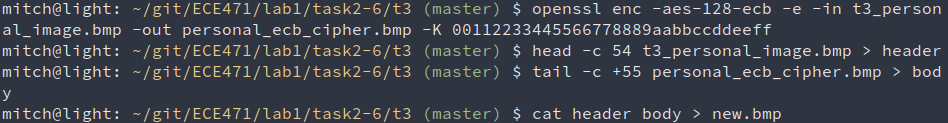
\includegraphics[scale=0.5]{t3p4.png}
    \end{center}{}
    \caption{Encrypting personal image using ECB}
    \label{fig:t3p4}
\end{figure}

Figure~\ref{fig:t3p4} shows the process of encrypting the personal image using ECB. This process is
very similar to Figure~\ref{fig:t3p2} and Figure~\ref{fig:t3p0}.

\begin{figure}[H]
    \begin{center}
        \includegraphics[scale=0.18]{t3_personal_ecb.jpg}
    \end{center}{}
    \caption{Result of encrypting with ECB}
    \label{fig:t3_personal_ecb}
\end{figure}

Figure~\ref{fig:t3_personal_ecb} shows the results of encrypting Figure~\ref{fig:t3_personal_image}
with ECB, which honestly is not too easy to identify what the image should be. This leads me to believe
that ECB only reveals the contents via inspection if there is a large enough contrast between objects
and colors.

\clearpage
\subsection{Task 4: Padding}

For block ciphers, when the size of a plaintext is not a multiple of the block size, padding
may be required. All the block ciphers normally use PKCS#5 padding, which is known as standard
block padding. We will conduct the following experiments to understand how this type of
padding works:
\begin{enumerate}
    \item Use ECB, CBC, CFB, and OFB modes to encrypt a file (you can pick any cipher). Please report
    which modes have paddings and which ones do not. For those that do not need paddings, please
    explain why.
    
    \item Let us create three files, which contain 5 bytes, 10 bytes, and 16 bytes, respectively. We
    can
    use the following "echo -n" command to create such files. The following example creates a file
    f1.txt with length 5 (without the -n option, the length will be 6, because a newline character will
    be added by echo):
    
\begin{verbatim}
$ echo -n "12345" > f1.txt
\end{verbatim}
    
    We then use "openssl enc -aes-128-cbc -e" to encrypt these three files using 128-bit AES with CBC
    mode. Please describe the size of the encrypted files. 
    
    We would like to see what is added to the padding during the encryption. To achieve this goal, we
    will decrypt these files using "openssl enc -aes-128-cbc -d". Unfortunately, decryption by default
    will automatically remove the padding, making it impossible for us to see the padding. However, the
    command does have an option called "-nopad", which disables the padding, i.e., during the
    decryption, the command will not remove the padded data. Therefore, by looking at the decrypted
    data, we can see what data are used in the padding. Please use this technique to figure out what
    paddings are added to the three files.

    It should be noted that padding data may not be printable, so you need to use a hex tool to display
    the content. The following example shows how to display a file in the hex format:
    
\begin{verbatim}
$ hexdump -C p1.txt
00000000 31 32 33 34 35 36 37 38 39 49 4a 4b 4c 0a  |123456789IJKL.|
$ xxd p1.txt
00000000: 3132 3334 3536 3738 3949 4a4b 4c0a         123456789IJKL.
\end{verbatim}
\end{enumerate}

\subsubsection{Task 4: Solution}
\begin{figure}[H]
    \begin{center}
        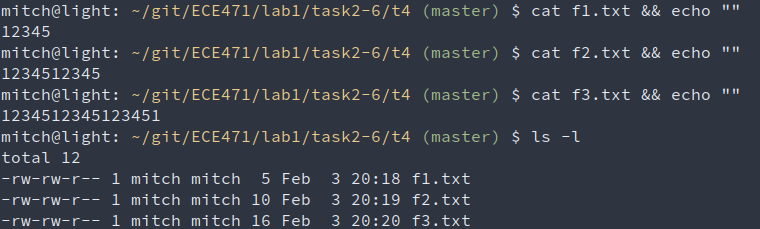
\includegraphics[scale=0.65]{t4p0.png}
    \end{center}{}
    \caption{task 4 test files}
    \label{fig:t4p0}
\end{figure}

Figure~\ref{fig:t4p0} shows the test files being used in this section. The files are very simple, and the linux command used shows the size of the files. f1.txt is 5 bytes, f2.txt is 10 bytes, and f3.txt is 16 bytes. Below is what the name of each of the encryption protocols we are using expands to.

\tab ECB - Electronic CodeBook \\
\tab CBC - Cipher-Block-Chaining \\
\tab CFB - Cipher-Feedback \\
\tab OFB - Output-FeedBack


To these three files, we need to encrypt and decrypt the file using ECB, CBC, CFB, and OFB. Because this is a lot of similar commands being utilized, a script was made to run this session. The script is copied below, and can be found in the most current state at \url{https://github.com/mitchdz/ECE471/blob/master/lab1/task2-6/t4/t4_commands.sh}.

\begin{verbatim}
#!/usr/bin/bash
KEY="00112233445566778889aabbccddeeff"
IV="01020304050607081234123412341212"
ENC_PREF="openssl enc -aes-128-"

CIPHER_PREF="cipher"
PLAIN_PREF="plain"
mkdir -p ${CIPHER_PREF}/
mkdir -p ${PLAIN_PREF}/

#encrypting
${ENC_PREF}ecb -e -in f1.txt -out ${CIPHER_PREF}/f1_ecb_cipher.txt -K ${KEY}
${ENC_PREF}ecb -e -in f2.txt -out ${CIPHER_PREF}/f2_ecb_cipher.txt -K ${KEY}
${ENC_PREF}ecb -e -in f3.txt -out ${CIPHER_PREF}/f3_ecb_cipher.txt -K ${KEY}
${ENC_PREF}cbc -e -in f1.txt -out ${CIPHER_PREF}/f1_cbc_cipher.txt -K ${KEY} \
    -iv ${IV}
${ENC_PREF}cbc -e -in f2.txt -out ${CIPHER_PREF}/f2_cbc_cipher.txt -K ${KEY} \
    -iv ${IV}
${ENC_PREF}cbc -e -in f3.txt -out ${CIPHER_PREF}/f3_cbc_cipher.txt -K ${KEY} \
    -iv ${IV}
${ENC_PREF}cfb -e -in f1.txt -out ${CIPHER_PREF}/f1_cfb_cipher.txt -K ${KEY} \
    -iv ${IV}
${ENC_PREF}cfb -e -in f2.txt -out ${CIPHER_PREF}/f2_cfb_cipher.txt -K ${KEY} \
    -iv ${IV}
${ENC_PREF}cfb -e -in f3.txt -out ${CIPHER_PREF}/f3_cfb_cipher.txt -K ${KEY} \
    -iv ${IV}
${ENC_PREF}ofb -e -in f1.txt -out ${CIPHER_PREF}/f1_ofb_cipher.txt -K ${KEY} \
    -iv ${IV}
${ENC_PREF}ofb -e -in f2.txt -out ${CIPHER_PREF}/f2_ofb_cipher.txt -K ${KEY} \
    -iv ${IV}
${ENC_PREF}ofb -e -in f3.txt -out ${CIPHER_PREF}/f3_ofb_cipher.txt -K ${KEY} \
    -iv ${IV}
#decrypting
${ENC_PREF}ecb -d -nopad -in ${CIPHER_PREF}/f1_ecb_cipher.txt \
    -out ${PLAIN_PREF}/f1_ecb_plain.txt -K ${KEY}
${ENC_PREF}ecb -d -nopad -in ${CIPHER_PREF}/f1_cbc_cipher.txt \
    -out ${PLAIN_PREF}/f1_cbc_plain.txt -K ${KEY}
${ENC_PREF}cfb -d -nopad -in ${CIPHER_PREF}/f1_cfb_cipher.txt \
    -out ${PLAIN_PREF}/f1_cfb_plain.txt -K ${KEY} -iv ${IV}
${ENC_PREF}ofb -d -nopad -in ${CIPHER_PREF}/f1_ofb_cipher.txt \
    -out ${PLAIN_PREF}/f1_ofb_plain.txt -K ${KEY} -iv ${IV}

${ENC_PREF}ecb -d -nopad -in ${CIPHER_PREF}/f2_ecb_cipher.txt \
    -out ${PLAIN_PREF}/f2_ecb_plain.txt -K ${KEY}
${ENC_PREF}cbc -d -nopad -in ${CIPHER_PREF}/f2_cbc_cipher.txt \
    -out ${PLAIN_PREF}/f2_cbc_plain.txt -K ${KEY} -iv ${IV}
${ENC_PREF}cfb -d -nopad -in ${CIPHER_PREF}/f2_cfb_cipher.txt \
    -out ${PLAIN_PREF}/f2_cfb_plain.txt -K ${KEY} -iv ${IV}
${ENC_PREF}ofb -d -nopad -in ${CIPHER_PREF}/f2_ofb_cipher.txt \
    -out ${PLAIN_PREF}/f2_ofb_plain.txt -K ${KEY} -iv ${IV}

${ENC_PREF}ecb -d -nopad -in ${CIPHER_PREF}/f3_ecb_cipher.txt \
    -out ${PLAIN_PREF}/f3_ecb_plain.txt -K ${KEY}
${ENC_PREF}cbc -d -nopad -in ${CIPHER_PREF}/f3_cbc_cipher.txt \
    -out ${PLAIN_PREF}/f3_cbc_plain.txt -K ${KEY} -iv ${IV}
${ENC_PREF}cfb -d -nopad -in ${CIPHER_PREF}/f3_cfb_cipher.txt \
    -out ${PLAIN_PREF}/f3_cfb_plain.txt -K ${KEY} -iv ${IV}
${ENC_PREF}ofb -d -nopad -in ${CIPHER_PREF}/f3_ofb_cipher.txt \
    -out ${PLAIN_PREF}/f3_ofb_plain.txt -K ${KEY} -iv ${IV}

#printing out results
echo "f1.txt"
printf "plain: "; xxd f1.txt
printf "ecb  : "; xxd plain/f1_ecb_plain.txt
printf "cbc  : "; xxd plain/f1_cbc_plain.txt
printf "cfb  : "; xxd plain/f1_cfb_plain.txt
printf "ofb  : "; xxd plain/f1_ofb_plain.txt

echo ""
echo "f2.txt"
printf "plain: "; xxd f2.txt
printf "ecb  : "; xxd plain/f2_ecb_plain.txt
printf "cbc  : "; xxd plain/f2_cbc_plain.txt
printf "cfb  : "; xxd plain/f2_cfb_plain.txt
printf "ofb  : "; xxd plain/f2_ofb_plain.txt

echo ""
echo "f3.txt"
printf "plain: "; xxd f3.txt
printf "ecb  : "; xxd plain/f3_ecb_plain.txt
printf "cbc  : "; xxd plain/f3_cbc_plain.txt
printf "cfb  : "; xxd plain/f3_cfb_plain.txt
printf "ofb  : "; xxd plain/f3_ofb_plain.txt

\end{verbatim}

\begin{figure}[H]
    \begin{center}
        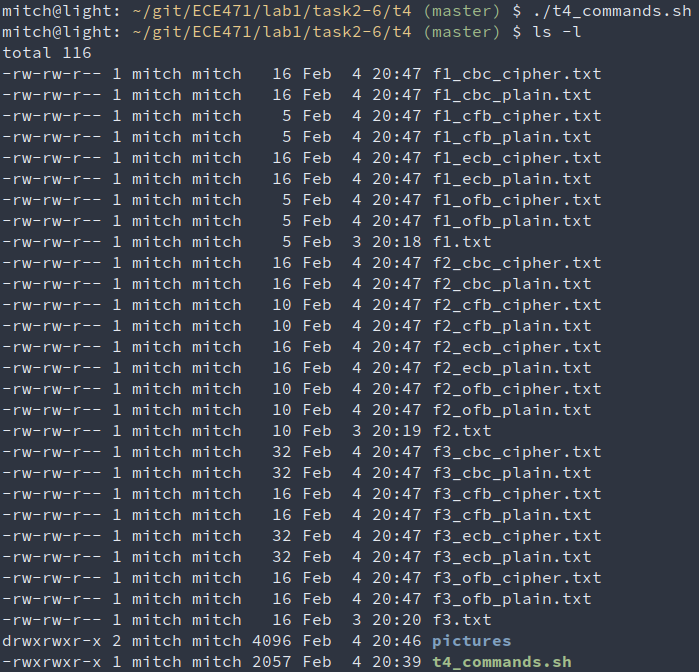
\includegraphics[scale=0.55]{t4p2.png}
    \end{center}{}
    \caption{task 4 script}
    \label{fig:t4p2}
\end{figure}

Figure~\ref{fig:t4p2} shows the resulting file sizes after executing the script made to encrypt and decrypt each file without removing the padding. Notice that cfb and ofb kept the file size the same for all three files. CBC and ECB however padded each file to either 16 or 32 bits.

Now to examine how the encryption schemes padded the file. Below is what the script outputs when ran from the directory.

\begin{verbatim}
mitch@light: ~/git/ECE471/lab1/task2-6/t4 (master) $ ./t4_commands.sh
f1.txt
plain: 00000000: 3132 3334 35                             12345
ecb  : 00000000: 3132 3334 350b 0b0b 0b0b 0b0b 0b0b 0b0b  12345...........
cbc  : 00000000: 3030 3030 300d 0c03 193f 193f 193f 1919  00000....?.?.?..
cfb  : 00000000: 3132 3334 35                             12345
ofb  : 00000000: 3132 3334 35                             12345

f2.txt
plain: 00000000: 3132 3334 3531 3233 3435                 1234512345
ecb  : 00000000: 3132 3334 3531 3233 3435 0606 0606 0606  1234512345......
cbc  : 00000000: 3132 3334 3531 3233 3435 0606 0606 0606  1234512345......
cfb  : 00000000: 3132 3334 3531 3233 3435                 1234512345
ofb  : 00000000: 3132 3334 3531 3233 3435                 1234512345

f3.txt
plain: 00000000: 3132 3334 3531 3233 3435 3132 3334 3531  1234512345123451
ecb  : 00000000: 3132 3334 3531 3233 3435 3132 3334 3531  1234512345123451
       00000010: 1010 1010 1010 1010 1010 1010 1010 1010  ................
cbc  : 00000000: 3132 3334 3531 3233 3435 3132 3334 3531  1234512345123451
       00000010: 1010 1010 1010 1010 1010 1010 1010 1010  ................
cfb  : 00000000: 3132 3334 3531 3233 3435 3132 3334 3531  1234512345123451
ofb  : 00000000: 3132 3334 3531 3233 3435 3132 3334 3531  1234512345123451
\end{verbatim}


As shown by the size of each file in the results of the bash script, OFB and CFB did not increase the size of the resulting plaintext, so the results shown in Figure~\ref{fig:t4p2} are as expected. However, ecb and cbc both padded the values to 16 bits, padding with the value `0b` over and over. The decimal equivalent of hex 0b is 11, which happens to be exactly the number of bytes that were used to pad the message! PKCS#5 pads the message repeatedly with the number of bytes required to pad the message.

f2.txt, the 10 byte file, has very similar results as f1.txt, however the major difference is the extra data is `0606` repeating. `06` in decimal is 6 which is the number of bytes added to the padding!

f3.txt, the 16 byte file, has very similar results as f1.txt and f2.txt, however the major difference is the extra data is an entire 16 bytes of `1010` repeating. It may seem fair to assume that no paddin gshould be done for ecb and cbc for this message because the message is 16 bytes. However, if the message itself ends with cewrtain bits that may look like it is being padded, part of the message may be lost. Therefore, the message is padded to the next multiple of 2 bytes, 32 bytes.


\clearpage
\subsection{Task 5: Error Propagation – Corrupted Cipher Text}
To understand the error propagation property of various encryption modes, we would like to do the
following exercise:
\begin{enumerate}
    \item Create a text file that is at least 1000 bytes long.
    \item Encrypt the file using the AES-128 cipher.
    \item Unfortunately, a single bit of the 55th byte in the encrypted file got corrupted. You can
    achieve this corruption using the bless hex editor.
    \item Decrypt the corrupted ciphertext file using the correct key and IV.
\end{enumerate}
\tab Please answer the following question: How much information can you recover by decrypting the corrupted file, if the encryption mode is ECB, CBC, CFB, or OFB, respectively? Please answer this question before you conduct this task, and then find out whether your answer is correct or wrong after you finish this task. Please provide justification.

\subsubsection{Task 5: Solution}

In order to create a file of at least 1000 bytes long, the only obvious choice was to use the bee movie. The file is found at this location - \url{https://github.com/mitchdz/ECE471/blob/master/lab1/task2-6/t5/bee_movie.txt}. The bee movie turns out to be 55394 bytes which is a lot more than 1000. Now the script needs to be encrypted using 128 bit AES. For this task, cbc is used.

\begin{verbatim}
mitch@light: ~/git/ECE471/lab1/task2-6/t5 (master) $ head bee_movie.txt
HOME
The Entire Bee Movie Script

Bee Movie Script - Dialogue Transcript


According to all known laws
of aviation,

\end{verbatim}

The first  9 lines of the bee movie are shown using the Linux `head` command.

Now the bee movie needs to be encrypted and decrypted using ECB, CBC, CFB, and OFB, then to see how much corrupting one bit changes the resulting plaintext when decrypted. 

Predictions: \\
    \tab ECB - not much change, mainly because the lack of difussion as shown in the previous tasks. \\
    \tab CBC - Not much change, simply because the algorithm is similar to ECB and works byte by byte, so the area where the bit is changed should look a lot different, but not the entire ciphertext.
    \tab CFB - A lot of change. CFB stands for Cipher Feedback, so the preceding blocks effect the future blocks.
    \tab OFB - A lot of change, similar to CFB. Same reasoning for CFB.

The procedure will be shown for CBC only, but know tha the procedure is the exact same for ECB, CBC, CFB, and OFB.

\begin{verbatim}
$ openssl enc -aes-128-cbc -e -in bee_movie.txt -out cipher.bin \
    -K 00112233445566778889aabbccddeeff \
    -iv 01020304050607081234123412341212
\end{verbatim}

The preceding command creates a file named cipher.bin. which is the encrypted file of the bee movie. Let's mess up a bit in the 55th byte of the bee movie now.

\begin{figure}[H]
    \begin{center}
        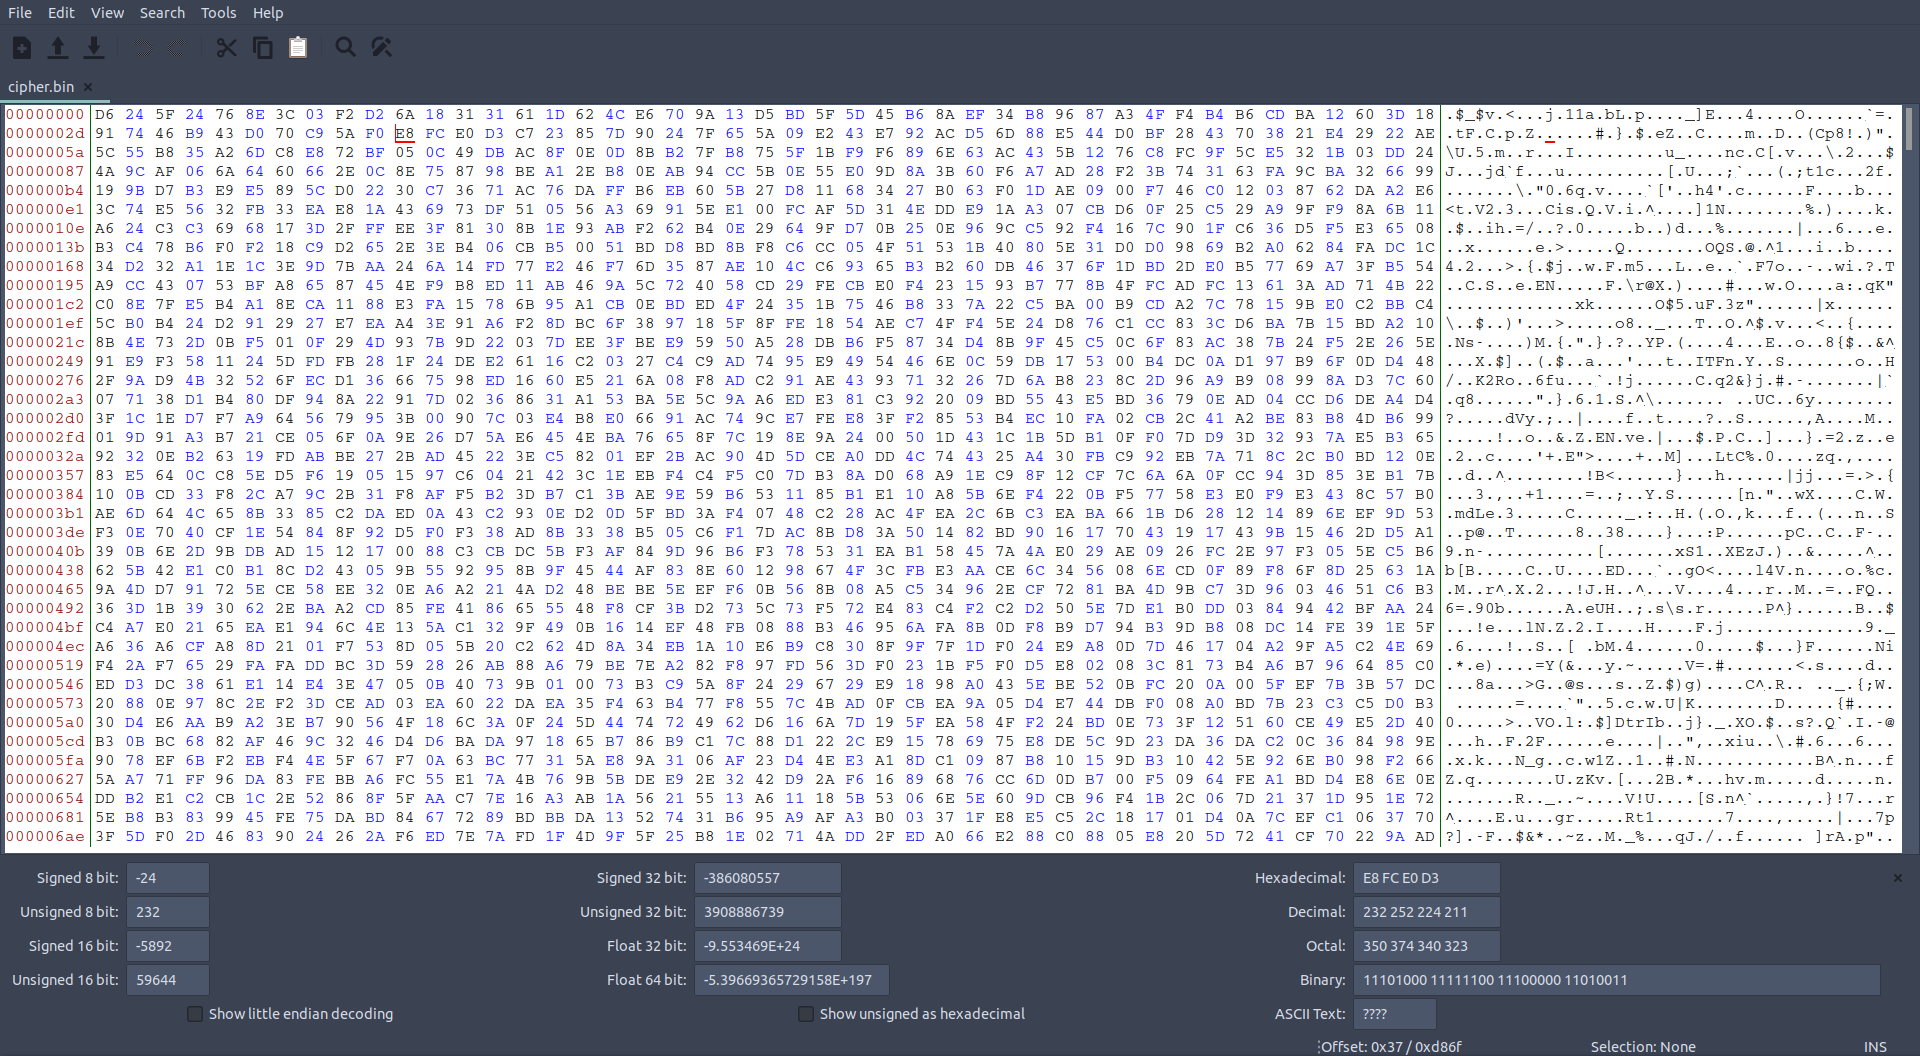
\includegraphics[scale=0.25]{t5p1.png}
    \end{center}{}
    \caption{bless editor showing bee movie encrypted with cbc}
    \label{fig:t5p1}
\end{figure}


Figure ~\ref{fig:t5p1} shows the bless hex editor viewing the bee movie encrypted using aes-128-cbc.

\begin{figure}[H]
    \begin{center}
        
\includegraphics[scale=1]{t5p1.1.png}
    \end{center}{}
    \caption{bless editor showing the offset}
    \label{fig:t5p1.1}
\end{figure}

Figure~\ref{fig:t5p1.1} shows Figure~\ref{fig:t5p1} zoomed in on the bottom right, where the bless hex editor shows the offset that your cursor is at. The offest is 0x37 because 0x37 in hex refers to 55 in decimal. 

0xE8 is at position 0x37 in bless, and 0xE8 is 232 in decimal. Let's change that value to 231, so that value is changed to E7 as shown in the following picture.

\begin{figure}[H]
    \begin{center}
        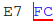
\includegraphics[scale=1]{t5p3.png}
    \end{center}{}
    \caption{Bless editor showing modified value at byte 0x37}
    \label{fig:t5p3}
\end{figure}

Figure~\ref{fig:t5p3} clearly shows the value is now E7. To save the file, press ctrl + c, and the file is saved! Now we need to decrypt the file. The following command is used in order to decrypt the file.

\begin{verbatim}
$ openssl enc -aes-128-cbc -d -in cipher.bin -out cbc_scrambled.txt \
    -K 00112233445566778889aabbccddeeff \
    -iv 01020304050607081234123412341212
\end{verbatim}


Now the head of each file is shown below.


\textbf{ECB:}
\begin{verbatim}
    HOME
    The Entire Bee Movie Script
    
    Bee Movie Scri#��>$�'��BA96�anscript
    
    
    According to all known laws
    of aviation,
\end{verbatim}

\textbf{CBC:}
\begin{verbatim}
    HOME
    The Entire Bee Movie Script
    
    Bee Movie Scri�)W�H�w/�,1���anscrip{
    
    
    According to all known laws
    of aviation,
\end{verbatim}

\textbf{CFB (shown as picture):}
\begin{figure}[H]
    \begin{center}
        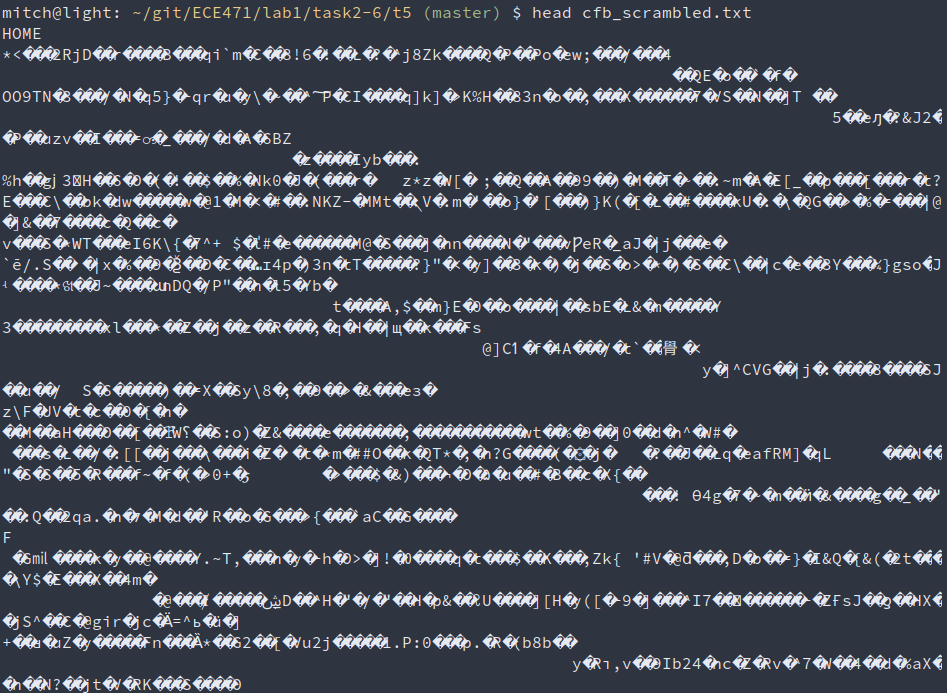
\includegraphics[scale=0.4]{t5p4.png}
    \end{center}{}
    \caption{Output of the plaintext after corrupting a bit using CFB}
    \label{fig:t5p4}
\end{figure}

\textbf{OFB:}
\begin{verbatim}
    HOME
    The Entire Bee Movie Script
    
    Bee Movie Script - Diflogue Transcript
    
    
    According to all known laws
    of aviation,
\end{verbatim}

Therefore, 3/4 of my predictions were correct! Figure~\ref{fig:t5p4} is shown as a picture because copying those characters broke LaTeX. Only CFB was majorly messed up. I was very surprised that OFB was not messed up because it is a stream cipher. This is because even though OFB is a cipher, the algorithm works like CBC/ECB because OFB streams the text BEFORE it is ciphertext. CFB encrypts the block and then pushes it through the stream. More information is found here on wikipedia \url{https://en.wikipedia.org/wiki/Block_cipher_mode_of_operation#Cipher_Feedback_(CFB)}.

\clearpage
\subsection{Task 6: Initial Vector (IV)}

Most of the encryption modes require an initial vector (IV). Properties of an IV depend on the cryptographic scheme used. If we are not careful in selecting IVs, the data encrypted by us may not be secure at all, even though we are using a secure encryption algorithm and mode. The objective of this task is to help students understand the problems if an IV is not selected properly. Please do the following experiments:

\begin{itemize}
    \item \textbf{Task 6.1.} A basic requirement for IV is uniqueness, which means that no IV may be reused under the same key. To understand why, please encrypt the same plaintext using (1) two different IVs, and (2) the same IV. Please describe your observation, based on which, explain why IV needs to be unique.
    \item \textbf{Task 6.2.} One may argue that if the plaintext does not repeat, using the same IV is safe. Let us look at the Output Feedback (OFB) mode. Assume that the attacker gets hold of a plaintext (P1) and a ciphertext (C1) , can he/she decrypt other encrypted messages if the IV is always the same? You are given the following information, please try to figure out the actual content of P2 based on C2, P1, and C1.
    
    \begin{verbatim}
    Plaintext (P1): This is a known message!
    Ciphertext (C1): a469b1c502c1cab966965e50425438e1bb1b5f9037a4c159
    Plaintext (P2): (unknown to you)
    Ciphertext (C2): bf73bcd3509299d566c35b5d450337e1bb175f903fafc159
    \end{verbatim}
        
    If we replace OFB in this experiment with CFB (Cipher Feedback), how much of P2 can be revealed? You only need to answer the question; there is no need to demonstrate that.
    
    The attack used in this experiment is called the known-plaintext attack, which is an attack model for cryptanalysis where the attacker has access to both the plaintext and its encrypted version (ciphertext). If this can lead to the revealing of further secret information, the encryption scheme is not considered as secure.
    
    \item \textbf{Task 6.3.} From the previous tasks, we now know that IVs cannot repeat. Another important requirement on IV is that IVs need to be unpredictable for many schemes, i.e., IVs need to be randomly generated. In this task, we will see what is going to happen if IVs are predictable.
    
    Assume that Bob just sent out an encrypted message, and Eve knows that its content is either Yes or No; Eve can see the ciphertext and the IV used to encrypt the message, but since the encryption algorithm AES is quite strong, Eve has no idea what the actual content is. However, since Bob uses predictable IVs, Eve knows exactly what IV Bob is going to use next. The following summarizes what Bob and Eve know:
    
    \begin{verbatim}
    Encryption method: 128-bit AES with CBC mode.
    Key (in hex): 00112233445566778899aabbccddeeff (known only to Bob)
    Ciphertext (C1): bef65565572ccee2a9f9553154ed9498 (known to both)
    IV used on P1 (known to both)
        (in ascii): 1234567890123456
        (in hex)  : 31323334353637383930313233343536
    Next IV (known to both)
        (in ascii): 1234567890123457
        (in hex)  : 31323334353637383930313233343537
    \end{verbatim}
    
    A good cipher should not only tolerate the known-plaintext attack described previously, it should also tolerate the chosen-plaintext attack, which is an attack model for cryptanalysis where the attacker can obtain the ciphertext for an arbitrary plaintext. Since AES is a strong cipher that can tolerate the chosen-plaintext attack, Bob does not mind encrypting any plaintext given by Eve; he does use a different IV for each plaintext, but unfortunately, the IVs he generates are not random, and they can always be predictable.
    
    Your job is to construct a message P2 and ask Bob to encrypt it and give you the ciphertext. Your objective is to use this opportunity to figure out whether the actual content of P1 is Yes or No. You can read this Wikipedia page for ideas: \url{https://en.wikipedia.org/wiki/Initialization_vector}.
\end{itemize}

    \tab There are more advanced cryptanalysis on IV that is beyond the scope of this lab. Students can read the article posted in this URL: \url{https://defuse.ca/cbcmodeiv.htm}. Because the requirements on IV really depend on cryptographic schemes, it is hard to remember what properties should be maintained when we select an IV. However, we will be safe if we always use a new IV for each encryption, and the new IV needs to be generated using a good pseudo random number generator, so it is unpredictable by adversaries. See another SEED labs (Random Number Generation Lab) for details on how to generate cryptographically strong pseudo random numbers.

\subsubsection{Task 6.1: Solution}

The plaintext is created using the Linux command echo, and then redirecting the output to a file.

\begin{verbatim}
$ echo "hello, I am a plaintext!" > plain.txt
\end{verbatim}

file 1.bin, 2.bin, and 3.bin are created in the following fashion:
\begin{verbatim}
$ openssl enc -aes-128-cbc -e -in plain.txt -out 1.bin \
    -K 00112233445566778889aabbccddeeff \
    -iv 01020304050607081234123412341212
\end{verbatim}
\begin{verbatim}
$ openssl enc -aes-128-cbc -e -in plain.txt -out 2.bin \
    -K 00112233445566778889aabbccddeeff \
    -iv 01020304050607081234123412341212
\end{verbatim}
\begin{verbatim}
$ openssl enc -aes-128-cbc -e -in plain.txt -out 3.bin \
    -K 00112233445566778889aabbccddeeff \
    -iv 00000000000000000000000000000000
\end{verbatim}

\begin{figure}[H]
    \begin{center}
        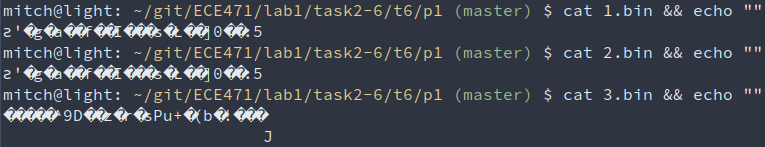
\includegraphics[scale=0.55]{t6p0.png}
    \end{center}{}
    \caption{Output of the three binary files from Task 2.6.1}
    \label{fig:t6p0}
\end{figure}

Figure ~\ref{fig:t6p0} shows the output of 1.bin, 2.bin, and 3.bin. 1.bin & 2.bin both used the same IV, whereas 3.bin used a different IV. It is apparent that 1.bin and 2.bin are the exact same file, which shows that using the same IV will result in the same ciphertext. This means that the ciphertext is repeatable, and if the same IV is used multiple times, it may be possible to determine what the IV is.
\clearpage
\subsubsection{Task 6.2: Solution}

In order to accomplish this task, the website \url{http://xor.pw/#} was used.

Output Feedback (OFB) is a stream cipher which relies heavily on XORing plaintext blocks with the key and an IV. If an IV and the key are the same for different plaintexts, it is trivial to decrypt P2 while utilizing a known-plaintext attack. The theory is outlined below:

\centering
K = P1 \bigoplus C1\\
P2 = K \bigoplus C2

\raggedright 
 
Let's see how well this theory holds up!

\begin{figure}[H]
    \begin{center}
        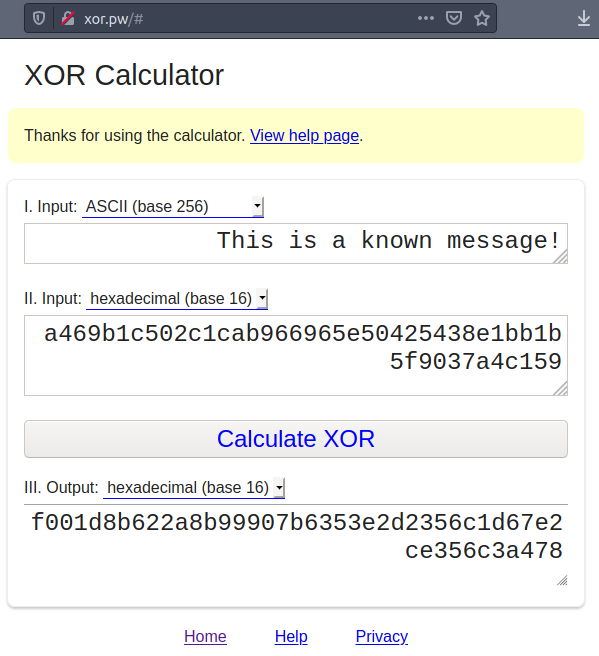
\includegraphics[scale=0.55]{t6p2.1.png}
    \end{center}{}
    \caption{Task 6.2: Finding K}
    \label{fig:t6p2.1}
\end{figure}

Figure~\ref{fig:t6p2.1} shows using \url{http://xor.pw/#} in order to calculate what K is. This website is great because we can directly XOR between ascii and hex, so there's no need to convert P1 to hex with another program first. The same operation is shown below in a format that is copy-able.

\begin{verbatim}
    This is a known message!                         (ascii)
XOR a469b1c502c1cab966965e50425438e1bb1b5f9037a4c159 (hex)
    ------------------------------------------------
    f001d8b622a8b99907b6353e2d2356c1d67e2ce356c3a478 (hex)
\end{verbatim}

Therefore, the key, K, is f001d8b622a8b99907b6353e2d2356c1d67e2ce356c3a478. Finding the plaintext associated with C2 is then trivial using the following operation.

\begin{figure}[H]
    \begin{center}
        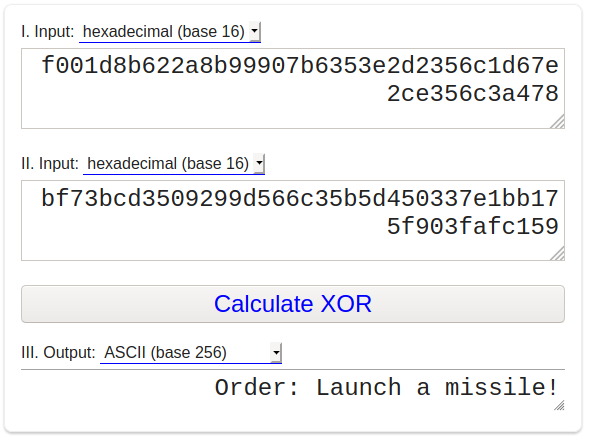
\includegraphics[scale=0.55]{t6p2.2.png}
    \end{center}{}
    \caption{Task 6.2: Decrypting C2}
    \label{fig:t6p2.2}
\end{figure}

Figure~\ref{fig:t6p2.2} shows deciphering C2 using the key found from Figure~\ref{fig:t6p2.1}! The resulting string is "Order: Launch a missile!". The XOR operation is shown below again.

\begin{verbatim}
    f001d8b622a8b99907b6353e2d2356c1d67e2ce356c3a478 (hex)
XOR bf73bcd3509299d566c35b5d450337e1bb175f903fafc159 (hex)
    ------------------------------------------------
    Order: Launch a missile!                         (ascii)
\end{verbatim}

P2 is therefore \textbf{Order: Launch a missile!}

For CFB, reusing an IV will leak some information about the first block of the plaintext. Any common prefix will also be leaked. CFB is a little bit more secure and will not completely break like OFB did.

\clearpage
\subsubsection{Task 6.3: Solution}

I choose my P2 to be the following:

\[ P2 = IV_{P1} \bigoplus IV_{P2} \bigoplus "No" \]

Bob will then encrypt the given P2 as such:

\[ C_2 = E_{k} (IV_2 \bigoplus P_2 ) = E_{k} (IV_2\bigoplus (IV_2\bigoplus IV_1 \bigoplus "No")) \]

$IV_1 \bigoplus IV_1$ cancel out, meaning that the operation that Bob ends up producing is the following:

\[ C_2 = E_k (IV_1 \bigoplus "No") \]

Now we should be able to compare $C_1$ and $C_2$ to see if they match! If they differ, then P1 says "Yes".

Therefore, carefully picking P2 will allow us to encrypt data through Bob using $IV_1$. $C_1 \bigoplus C_2$ = 0x1 because the difference between them is just one number. Therefore the P2 when we use "No" as our reference is calculated as the following:

\begin{verbatim}
    no (ascii)
XOR 1  (hex)
    -----------
    Nn (Ascii)
\end{verbatim}

The above operation shows that \textbf{P2 shall be chosen to be "Nn"}. The following commands are used to demonstrate this chosen-plaintext attack.

\begin{verbatim}
echo "Nn" > P2
openssl enc -aes-128-cbc -e -in P2 -out P2.bin\
    -K  00112233445566778899aabbccddeeff \
    -iv 31323334353637383930313233343537
xxd -p P2.bin

\end{verbatim}

The end result after executing that command is 04a7ae2040bf474ce8bd33bec3165370 which is a lot different than C1 which is (bef65565572ccee2a9f9553154ed9498).

Therefore, P1 is "Yes".

\end{document}
